\begin{enumerate}[label=\thechapter.\arabic*,ref=\thechapter.\theenumi]

\item The number of zeroes of the polynomial $P(s) = s^3+2s^2+5s+80$ in the right side of the plane?\hfill(GATE IN 2023) \\

\solution
\iffalse
\let\negmedspace\undefined
\let\negthickspace\undefined
\documentclass[journal,12pt,twocolumn]{IEEEtran}
\usepackage{cite}
\usepackage{amsmath,amssymb,amsfonts,amsthm}
\usepackage{algorithmic}
\usepackage{graphicx}
\usepackage{textcomp}
\usepackage{xcolor}
\usepackage{txfonts}
\usepackage{listings}
\usepackage{enumitem}
\usepackage{mathtools}
\usepackage{gensymb}
\usepackage{comment}
\usepackage[breaklinks=true]{hyperref}
\usepackage{tkz-euclide} 
\usepackage{listings}
\usepackage{gvv} 
\usepackage{caption}
\def\inputGnumericTable{}                   

%\usepackage[latin1]{inputenc}                                
\usepackage{color}                                            
\usepackage{array}                                            
\usepackage{longtable}                                       
\usepackage{calc}                                             
\usepackage{multirow}                                         
\usepackage{hhline}                                           
\usepackage{ifthen}                                           
\usepackage{lscape}

\newtheorem{theorem}{Theorem}[section]
\newtheorem{problem}{Problem}
\newtheorem{proposition}{Proposition}[section]
\newtheorem{lemma}{Lemma}[section]
\newtheorem{corollary}[theorem]{Corollary}
\newtheorem{example}{Example}[section]
\newtheorem{definition}[problem]{Definition}
\newcommand{\BEQA}{\begin{eqnarray}}
\newcommand{\EEQA}{\end{eqnarray}}
\newcommand{\define}{\stackrel{\triangle}{=}}
\theoremstyle{remark}
\newtheorem{rem}{Remark}

\begin{document}

\bibliographystyle{IEEEtran}
\vspace{3cm}

\title{GATE: IN - 24.2023}
\author{EE23BTECH11013 - Avyaaz$^{*}$% <-this % stops a space 
}
\maketitle
\newpage
\bigskip

\renewcommand{\thefigure}{\arabic{figure}}
\renewcommand{\thetable}{\arabic{table}}

\large\textbf{\textsl{Question:}}
The number of zeroes of the polynomial $P(s) = s^3+2s^2+5s+80$ in the right side of the plane?\hfill(GATE IN 2023) \\
\solution
\fi
The table below shows the Routh array of the $n^{th}$- order characteristic polynomial : 
\begin{align}
    a_0s^n+a_1s^{n-1}......+a_{n-1}s^1+a_ns^0
\end{align}

\begin{table}[htbp]
\setlength{\extrarowheight}{8pt}
\centering
\begin{tabular}{|c|c|c|c|c|}
\hline 
$s^n$ & $ a_0 $ & $a_2 $ &  $a_4$ & ... \\
\hline
$s^{n-1}$ &$a_1$&$a_3$&$a_5$&...  \\
\hline
$s^{n-2} $& $b_1 = \dfrac{a_1a_2-a_3a_0}{a_1}$ &$b_2 = \dfrac{a_1a_4 - a_5a_0}{a_1}$ &...&..\\
\hline
$s^{n-3} $& $c_1 = \dfrac{b_1a_3-b_2a_1}{b_1}$  & $\vdots$ && \\
\hline
$\vdots$ & $\vdots$ & $\vdots$&&\\
\hline
$s^1$&$\vdots$&$\vdots$&&\\
\hline
$s^0$&$a_n$&&&\\
\hline
\end{tabular}

\caption{Routh Array}
\label{tab:routharray.IN.24.2023}
\end{table}
 Characteristic Equation:
\begin{align}
   s^3+2s^2+5s+80 = 0  
\end{align}


\noindent From \tabref{tab:routharray.IN.24.2023}:

\begin{table}[htbp]
\setlength{\extrarowheight}{10pt}
\centering
\begin{tabular}{|c|c|c|}
\hline 
$s^3$ & $ 1 $ & $5$ \\
\hline
$s^2$ &$2$&$80$ \\
\hline
$s^1 $& $\dfrac{2\times 5-80\times1}{2}= 
 -35$ & \\
\hline
$s^0 $& $ \dfrac{-35 \times 80}{-35} = 80$ &\\
\hline
\end{tabular}

\caption{}
\label{tab:inputs.IN.24.2023}
\end{table}

% The number of sign changes of the terms of the first column of the Routh Array corresponds to the number of roots of the characteristic equation in the right half of the s-plane.

\noindent From \tabref{tab:inputs.IN.24.2023}:

Since there are 2 sign changes in the first column of the Routh tabulation. So, the number of zeros in the right
half of the s-plane will be 2.

% s1 = -4.63925
% s2 = 1.31963 + 3.93735 i
% s3 = 1.31963 - 3.93735 i
% A pole is a value of s (in the Laplace domain) for which the transfer function becomes infinite.
% A zero is a value of s for which the transfer function becomes zero.

% In the Laplace domain, a transfer function 
% H(s) is typically represented as a ratio of polynomials in s: H(s)= N(s)/D(s)

\begin{figure}[htbp]
    \centering
    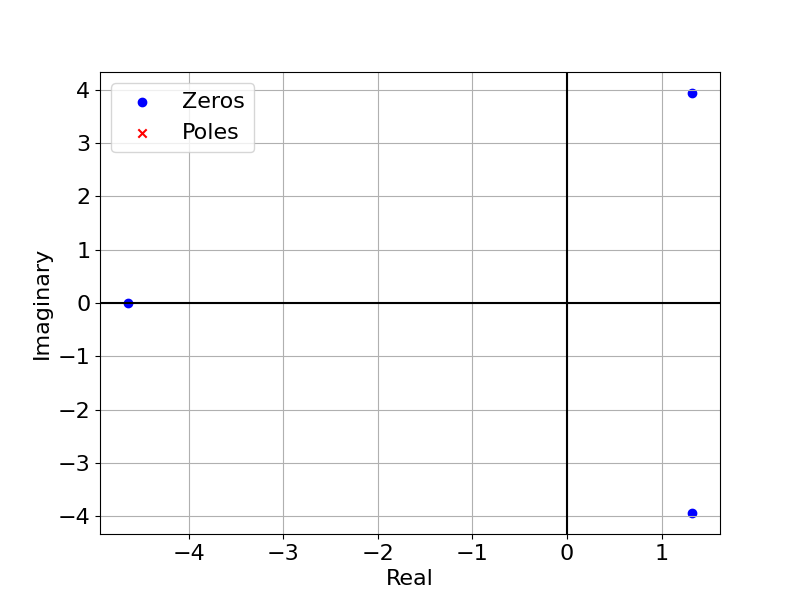
\includegraphics[width = \columnwidth]{2023/IN/24/figs/poles and root_plot.png}
  \caption{}
    \label{fig:graph1}
\end{figure}

% \bibliographystyle{IEEEtran}

\newpage

\item The circuit shown in the figure is initially in the steady state with the switch K in open condition and $\overline{K}$ in closed condition. The switch K is closed and $\overline{K}$ is opened simultaneously at the instant $t = t_1$, where $t_1 > 0$. The minimum value of $t_1$ in milliseconds such that there is no transient in the voltage across the 100 $\mu F$ capacitor, is \rule{1cm}{0.15mm} (Round off to 2 decimal places) \hfill (GATE EE 2023)
    \begin{circuitikz}[american]
        \draw (0,7) to [R=10$\Omega$] (0,2) to [short] (3.5,2) to [isource, l={$\sin\brak{1000t}$}] (3.5,7) to [short] (0,7);
        \draw (3.5,2) to [short] (5,2) to [short] (5,0) to [R=$10\Omega$] (7.5,0) to [battery2 = 5V] (10,0) to [short] (10,2) to [curved capacitor=100$\mu$F, invert] (10,7) to [short] (5,7) to [short] (3.5,7);
        \draw (5,2) to [short] (7, 2) to[ospst=$\overline{K}$] ++(1,0);
        \draw (5,5) to [short] (5,2);
        \draw (10,2) to [short] (8,2);
        \draw (5,7) to [short] (5,6) to[cspst=K] ++(0,-1) ;
\end{circuitikz}
\\
\solution
\iffalse
\documentclass[journal,12pt,twocolumn]{IEEEtran}
\usepackage{amsmath,amssymb,amsfonts,amsthm}
\usepackage{txfonts}
\usepackage{tkz-euclide}
\usepackage{listings}
\usepackage{gvv}
\usepackage[latin1]{inputenc}
\usepackage{adjustbox}
\usepackage{array}
\usepackage{tabularx}
\usepackage{pgf}
\usepackage{lmodern}
\usepackage{circuitikz}
\usepackage{tikz}
\usepackage{graphicx}

\begin{document}
\bibliographystyle{IEEEtran}

\vspace{3cm}

\title{}
\author{EE23BTECH11054 -  Sai Krishna Shanigarapu$^{*}$
}
\maketitle
\newpage
\bigskip

% \renewcommand{\thefigure}{\theenumi}
% \renewcommand{\thetable}{\theenumi}

\section*{Gate EE 2023}
54. \hspace{2pt}The circuit shown in the figure is initially in the steady state with the switch K in open condition and $\overline{K}$ in closed condition. The switch K is closed and $\overline{K}$ is opened simultaneously at the instant $t = t_1$, where $t_1 > 0$. The minimum value of $t_1$ in milliseconds such that there is no transient in the voltage across the 100 $\mu F$ capacitor, is \rule{1cm}{0.15mm} (Round off to 2 decimal places).\\ 
\hfill(GATE EE 2023)

\begin{figure}[ht]
  \centering
  \begin{adjustbox}{width=1\columnwidth}
          \begin{circuitikz}[american]
        \draw (0,7) to [R=10$\Omega$] (0,2) to [short] (3.5,2) to [isource, l={$\sin\brak{1000t}$}] (3.5,7) to [short] (0,7);
        \draw (3.5,2) to [short] (5,2) to [short] (5,0) to [R=$10\Omega$] (7.5,0) to [battery2 = 5V] (10,0) to [short] (10,2) to [curved capacitor=100$\mu$F, invert] (10,7) to [short] (5,7) to [short] (3.5,7);
        \draw (5,2) to [short] (7, 2) to[ospst=$\overline{K}$] ++(1,0);
        \draw (5,5) to [short] (5,2);
        \draw (10,2) to [short] (8,2);
        \draw (5,7) to [short] (5,6) to[cspst=K] ++(0,-1) ;
\end{circuitikz}

  \end{adjustbox}
  \caption{Circuit 1}
\end{figure}

\solution
\fi
\begin{enumerate}
\item Switch K is open and $\overline{K}$ is closed.

\begin{figure}[ht]
  \centering
          \begin{circuitikz}[american]
        \draw (0,7) to [R=10$\Omega$] (0,2) to [short] (3,2) to [isource, l=$1\angle{0^\circ}$] (3,7) to [short] (0,7);
        \draw (3,7) to [short, i=$I_1$] (7,7);
        \draw (3,2) to [short] (7,2);
        \draw (7,7) -- ++(0,-1.5)
        to [open, v=$V_1$, o-o] ++(0,-1.5) -- ++(0,-2);
\end{circuitikz}


  \caption{K is open and $\overline{K}$ is closed}
\end{figure}


Using Current divider rule,
\begin{align}
   I_1\brak{j\omega} &= \frac{10}{10+\frac{1}{j\omega C}}\\
   V_1\brak{j\omega} &= \frac{10}{1+10j\omega C}\\
   \abs{V_1\brak{j\omega}} &= 5\sqrt{2}
 \end{align}
 From Table \ref{tab:Gate.ee.54.1}
 \begin{align}
   V_1\brak{t} &= 5\sqrt{2}\sin\brak{\omega t - \frac{\pi}{4}} \label{eq:1.gate.ee.23.54}
\end{align}


\item Switch K is closed and $\overline{K}$ is open.


\begin{figure}[ht]
  \centering
      %\begin{circuitikz}[american]
        %\draw (0,0) to [R=10$\Omega$] (1.5,0) to [battery2=5V] (4,0);
        %\draw (0,0) to [short] (0,3) to [short] (4,3) to [C=100$\mu$F, %v=$V_c\brak{\infty}$] (4,0) ;
%\end{circuitikz}

\begin{circuitikz}[american]
    \draw (0,0) to [R=10$\Omega$] (1.5,0) to [battery2=$\frac{5}{s}$] (4,0);
    \draw[<-, thick] (1.5,1) arc (-90:90:0.5) node[midway, left] {$I(s)$};
    \draw (0,0) to [short] (0,3) to [short] (4,3) to [C=$\frac{10^4}{s}$, v=$V_c\brak{s}$] (4,0);
\end{circuitikz}


  \caption{K is closed and $\overline{K}$ is open}
\end{figure}
}


The capacitor is charged. Thus, acts as a voltage source.\\
From eq\brak{\ref{eq:1.gate.ee.23.54}} and Table \ref{tab:Gate.ee.54.2}
\begin{align}
    V_1\brak{s} &= \frac{5000 - 5s}{s^2 + 10^6} \\
    I\brak{s} &= \frac{\frac{5}{s} - V_1\brak{s}}{10 + \frac{10^4}{s}}\\
    V_c\brak{s} &= \frac{5}{s} - 10\brak{\frac{5-V_1\brak{s}}{1+10^{-3}s}}
\end{align}
\end{enumerate}

For transient analysis,
\begin{align}
    \frac{5-V_1\brak{s}}{1+10^{-3}s} &= 0\\
    \implies V_1\brak{s} &= 5\\
    \frac{10^7}{\brak{s^2+10^6}\brak{s+10^3}} &= \frac{5}{s}\\
    \frac{5}{s+10^3} + \frac{10^3-s}{s^2 + 10^6} &= \frac{5}{s}\\
    \frac{-s}{s^2+10^6} + \frac{10^3}{s^2 + 10^6} + \frac{1}{s+10^3} &= \frac{1}{s}
\end{align}
From Table \ref{tab:Gate.ee.54.2}
\begin{align}
    -\cos\brak{1000t_1}+\sin\brak{1000t_1}+e^{-10^3 t_1} &= 1\\
    \implies t_1 \approx 1.57\text{msec}
\end{align}

\begin{table}[ht]
       \setlength{\arrayrulewidth}{0.3mm}
\setlength{\tabcolsep}{20pt}
\renewcommand{\arraystretch}{1.3}



\begin{tabular}{|c|c|c|}
\hline

Parameter& Description & Remarks\\
\hline
$\omega$ & frequency of sine-wave & 1000 rad s$^{-1}$\\
\hline
$V_1\brak{t}$ & Voltage across capacitor & $\abs{V_1\brak{j\omega}}\sin\brak{\omega t - \angle{V_1\brak{j\omega}}}$\\
\hline
$\angle{V_1\brak{j\omega}} $ & phase of $V_1\brak{j\omega}$ & $\frac{-\pi}{4}$\\
\hline
$C$ & Capacitance & 100$\mu$F\\
\hline

\end{tabular}






    \caption{Parameters}
    \label{tab:Gate.ee.54.1}

\end{table}


\begin{table}[ht]
    \setlength{\arrayrulewidth}{0.3mm}
\setlength{\tabcolsep}{20pt}
\renewcommand{\arraystretch}{1.3}


\begin{tabular}{|c|c|}
\hline

S Domain & Time Domain\\
\hline
$\frac{1}{s}$ & $u\brak{t}$\\
\hline
$\frac{-s}{a^2+s^2}$ & $-\cos\brak{at}$\\
\hline
$\frac{a}{a^2+s^2}$ & $\sin\brak{at}$\\
\hline
$\frac{1}{s+a}$ & $e^{-at}$\\
\hline

\end{tabular}





    \caption{Laplace transforms}
    \label{tab:Gate.ee.54.2}
\end{table}

\begin{figure}[htbp]
    \centering
    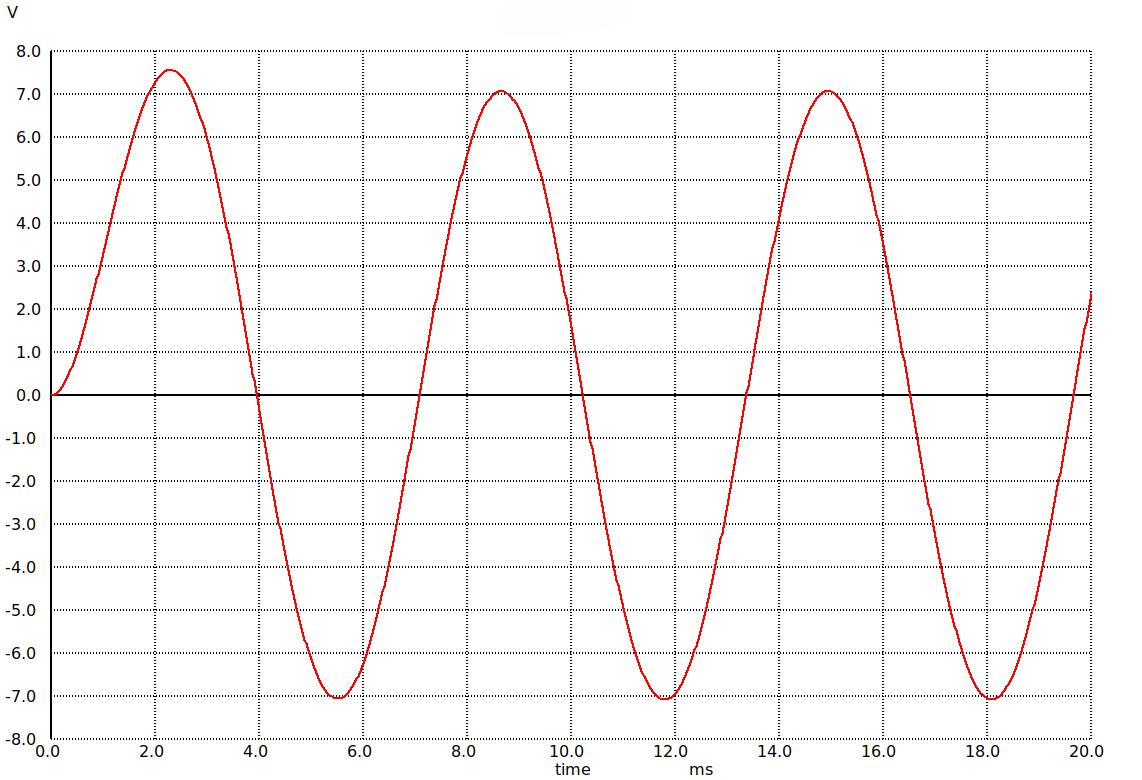
\includegraphics[width=1\columnwidth]{2023/EE/54/figs/fig1.png}
    \caption{plot of $V_1$ vs time}
\end{figure}

\begin{figure}[htbp]
    \centering
    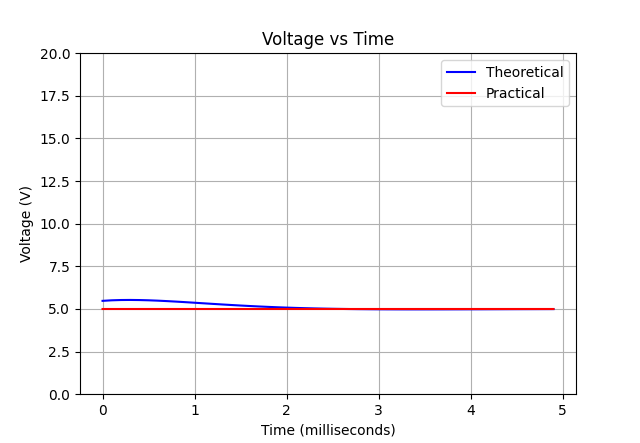
\includegraphics[width=1\columnwidth]{2023/EE/54/figs/fig3.png}
    \caption{plot of $V_c$ vs time}
\end{figure}

%\end{document}


\newpage
\item $y=e^{mx}+e^{-mx}$ is the solution of which differential equation?
\begin{enumerate}[label=\textbf{\arabic*.}, font=\bfseries, align=left]
    \item $\frac{dy}{dx} - my = 0$ 
    \item $\frac{dy}{dx} + my = 0$ 
    \item $\frac{d^{2}y}{dx^{2}} + m^{2}y = 0$ 
    \item $\frac{d^{2}y}{dx^{2}} - m^{2}y = 0$ 
\end{enumerate} \hfill(GATE AG 2023)
\solution

\newpage
\item  A cascade control strategy is shown in the figure below. The transfer function between the output $(y)$ and the secondary disturbance $(d_2)$ is defined as  \\
$$G_{d2}(s)= \frac{y(s)}{d_2(s)}$$. 
Which one of the following is the CORRECT expression for the transfer function $G_{d2}(s)$? \\
\begin{figure}[h]
    \centering
    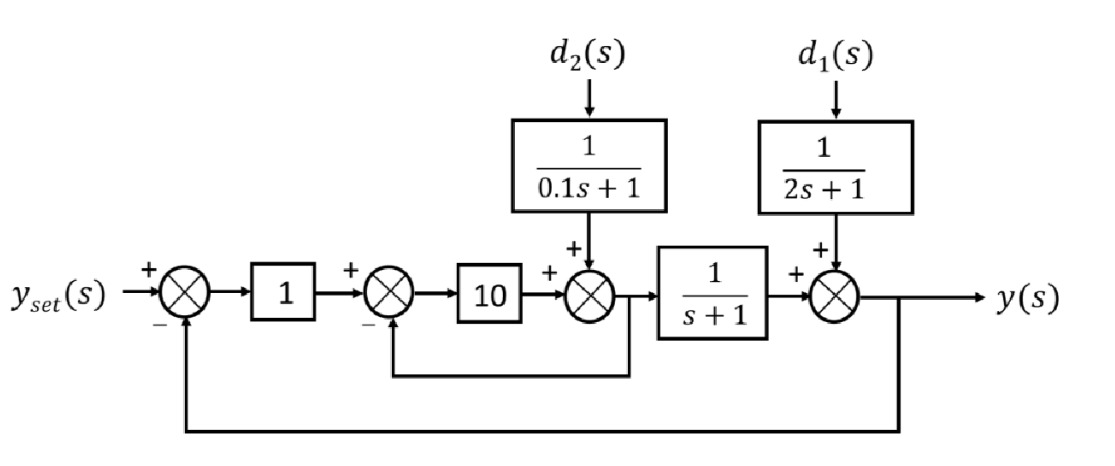
\includegraphics[scale=0.25]{2023/CH/44/figs/g44fig1.jpeg}
    \caption{ }
    \label{}
\end{figure}
\begin{enumerate}[label=\Alph*.]
\item $\frac{1}{(11s+21)(0.1s+1)}$ 
\item $\frac{1}{(s+1)(0.1s+1)}$
\item $\frac{(s+1)}{(s+2)(0.1s+1)}$
\item $\frac{(s+1)}{(s+1)(0.1s+1)}$
\end{enumerate} \hfill (GATE CH 2023)
\solution
\newpage
\item In the differential equation $\frac{dy}{dx} + \alpha x y = 0, \alpha$ is a positive constant. If $y = 1.0$ at
$x = 0.0$, and $y = 0.8$ at $x = 1.0$, the value of $\alpha$ is (rounded off to three decimal places).  \hfill(GATE CE 2023)
\solution

\newpage
\item The switch $S_1$ was closed and $S_2$ was open for a long time. At t=0,switch $S_1$ is opened and $S_2$ is closed,simultaneously. The value of $i_c(0^{+})$, in amperes, is . \hfill (GATE EC 2023)\\
\begin{circuitikz}[american]
   \draw (0,0) to [isource, l=1A] (0,4) ;
   \draw (0,0) to [short] (3,0) to [C = 0.01F] (3,4) to [short] (6,4) to [R = 100 $\Omega$] (6,2) to [L = 1H] (6,0) to [short] (9,0) to [R = 25 $\Omega$] (9,4) to [short] (6,4) ;
   \draw (3,0) to [short] (6,0) ;
   \draw (0,4) to [ospst = $S_1$] ++(3,0); 
   \draw (7.5,4) to [cspst = $S_2$] ++(0,-2);
   \draw (7.5,2) to [short] (6,2) ;
   \draw (3,4) to [short ,i = $i_c$] (3,3);
   
\end{circuitikz}

\newpage

\item The continuous time signal $x(t)$ is described by:
\begin{align}
x(t)=
    \begin{cases}
        1, & \text{if } 0\: {\displaystyle \leq }\:t\:{\displaystyle \leq }\:1\\
        0, & \text{elsewhere}
    \end{cases} 
\end{align}
If $y(t)$ represents $x(t)$ convolved with itself, which of the following options is/are TRUE?
\begin{enumerate}[label = \Alph*]
    \item $y(t)$ = 0 for all $t<0$\\
    \item $y(t)$ = 0 for all $t>1$\\
    \item $y(t)$ = 0 for all $t>3$\\
    \item $\int_{0.1}^{0.75} \frac{dy(t)}{dt}\: \text{dt} \neq 0$
\end{enumerate}
\solution
\newpage

\item The Z-transform of a discrete signal $x\brak{n}$ is
\begin{align}
X\brak{z}=\dfrac{4z}{\brak{z-\dfrac{1}{5}} \brak{z-\dfrac{2}{3}} \brak{z-3}} \text{ with ROC= }R
\end{align}
Which one of the following statements is TRUE?
\begin{enumerate}[label = (\alph*)]
     \item Discrete time Fourier transform of $x\sbrak{n}$ converges if $R$ is $|z|>3$\\
     \item Discrete time Fourier transform of $x\sbrak{n}$ converges if $ R$ is $\dfrac{2}{3}<|z|<3$\\
     \item Discrete time Fourier transform of $x\sbrak{n}$ converges if $R$ is such that $x\sbrak{n}$ is a left-sided sequence.\\
     \item Discrete time Fourier transform of $x\sbrak{n}$ converges if $R$ is such that $x\sbrak{n}$is a right-sided sequence.\\
 \end{enumerate} \hfill{GATE EE 2023}	\\
 \solution
 %\iffalse
\let\negmedspace\undefined
\let\negthickspace\undefined
\documentclass[journal,12pt,twocolumn]{IEEEtran}
\usepackage{cite}
\usepackage{amsmath,amssymb,amsfonts,amsthm}
\usepackage{algorithmic}
\usepackage{graphicx}
\usepackage{textcomp}
\usepackage{xcolor}
\usepackage{txfonts}
\usepackage{listings}
\usepackage{enumitem}
\usepackage{mathtools}
\usepackage{gensymb}
\usepackage{comment}
\usepackage[breaklinks=true]{hyperref}
\usepackage{tkz-euclide} 
\usepackage{listings}
\usepackage{gvv}  
\usepackage{tikz}
\usepackage{circuitikz} 
\usepackage{caption}

\def\inputGnumericTable{}                                
\usepackage[latin1]{inputenc}                 
\usepackage{color}                            
\usepackage{array}                            
\usepackage{longtable}                        
\usepackage{calc}                            
\usepackage{multirow}                      
\usepackage{hhline}                           
\usepackage{ifthen}                          
\usepackage{lscape}
\usepackage{amsmath}
\newtheorem{theorem}{Theorem}[section]
\newtheorem{problem}{Problem}
\newtheorem{proposition}{Proposition}[section]
\newtheorem{lemma}{Lemma}[section]
\newtheorem{corollary}[theorem]{Corollary}
\newtheorem{example}{Example}[section]
\newtheorem{definition}[problem]{Definition}
\newcommand{\BEQA}{\begin{eqnarray}}
\newcommand{\EEQA}{\end{eqnarray}}
\newcommand{\define}{\stackrel{\triangle}{=}}
\theoremstyle{remark}
\newtheorem{rem}{Remark}


\begin{document}
%

\bibliographystyle{IEEEtran}


\vspace{3cm}

\title{
%	\logo{
GATE EE 2023 

\large{EE:1205 Signals and System}

Indian Institute of Technology, Hyderabad
%	}
}
\author{Prashant Maurya

EE23BTECH11218
}	
%\title{
%	\logo{Matrix Analysis through Octave}{\begin{center}\includegraphics[scale=.24]{tlc}\end{center}}{}{HAMDSP}
%}


% paper title
% can use linebreaks \\ within to get better formatting as desired
%\title{Matrix Analysis through Octave}
%
%
% author names and IEEE memberships
% note positions of commas and nonbreaking spaces ( ~ ) LaTeX will not break
% a structure at a ~ so this keeps an author's name from being broken across
% two lines.
% use \thanks{} to gain access to the first footnote area
% a separate \thanks must be used for each paragraph as LaTeX2e's \thanks
% was not built to handle multiple paragraphs
%

%\author{<-this % stops a space
%\thanks{}}
%}
% note the % following the last \IEEEmembership and also \thanks - 
% these prevent an unwanted space from occurring between the last author name
% and the end of the author line. i.e., if you had this:
% 
% \author{....lastname \thanks{...} \thanks{...} }
%                     ^------------^------------^----Do not want these spaces!
%
% a space would be appended to the last name and could cause every name on that
% line to be shifted left slightly. This is one of those "LaTeX things". For
% instance, "\textbf{A} \textbf{B}" will typeset as "A B" not "AB". To get
% "AB" then you have to do: "\textbf{A}\textbf{B}"
% \thanks is no different in this regard, so shield the last } of each \thanks
% that ends a line with a % and do not let a space in before the next \thanks.
% Spaces after \IEEEmembership other than the last one are OK (and needed) as
% you are supposed to have spaces between the names. For what it is worth,
% this is a minor point as most people would not even notice if the said evil
% space somehow managed to creep in.



% The paper headers
%\markboth{Journal of \LaTeX\ Class Files,~Vol.~6, No.~1, January~2007}%
%{Shell \MakeLowercase{\textit{et al.}}: Bare Demo of IEEEtran.cls for Journals}
% The only time the second header will appear is for the odd numbered pages
% after the title page when using the twoside option.
% 
% *** Note that you probably will NOT want to include the author's ***
% *** name in the headers of peer review papers.                   ***
% You can use \ifCLASSOPTIONpeerreview for conditional compilation here if
% you desire.




% If you want to put a publisher's ID mark on the page you can do it like
% this:
%\IEEEpubid{0000--0000/00\$00.00~\copyright~2007 IEEE}
% Remember, if you use this you must call \IEEEpubidadjcol in the second
% column for its text to clear the IEEEpubid mark.



% make the title area
\maketitle

\newpage

%\tableofcontents

\bigskip

\renewcommand{\thefigure}{\arabic{figure}}
\renewcommand{\thetable}{\arabic{table}}
%\renewcommand{\theequation}{\theenumi}

%\begin{abstract}
%%\boldmath
%In this letter, an algorithm for evaluating the exact analytical bit error rate  (BER)  for the piecewise linear (PL) combiner for  multiple relays is presented. Previous results were available only for upto three relays. The algorithm is unique in the sense that  the actual mathematical expressions, that are prohibitively large, need not be explicitly obtained. The diversity gain due to multiple relays is shown through plots of the analytical BER, well supported by simulations. 
%
%\end{abstract}
% IEEEtran.cls defaults to using nonbold math in the Abstract.
% This preserves the distinction between vectors and scalars. However,
% if the journal you are submitting to favors bold math in the abstract,
% then you can use LaTeX's standard command \boldmath at the very start
% of the abstract to achieve this. Many IEEE journals frown on math
% in the abstract anyway.

% Note that keywords are not normally used for peerreview papers.
%\begin{IEEEkeywords}
%Cooperative diversity, decode and forward, piecewise linear
%\end{IEEEkeywords}



% For peer review papers, you can put extra information on the cover
% page as needed:
% \ifCLASSOPTIONpeerreview
% \begin{center} \bfseries EDICS Category: 3-BBND \end{center}
% \fi
%
% For peerreview papers, this IEEEtran command inserts a page break and
% creates the second title. It will be ignored for other modes.
%\IEEEpeerreviewmaketitle	
\textbf{Question: }The Z-transform of a discrete signal $x\brak{n}$ is
\begin{align}
X\brak{z}=\dfrac{4z}{\brak{z-\dfrac{1}{5}} \brak{z-\dfrac{2}{3}} \brak{z-3}} \text{ with ROC= }R
\end{align}
Which one of the following statements is TRUE?
\begin{enumerate}[label = (\alph*)]
     \item Discrete time Fourier transform of $x\sbrak{n}$ converges if $R$ is $|z|>3$\\
     \item Discrete time Fourier transform of $x\sbrak{n}$ converges if $ R$ is $\dfrac{2}{3}<|z|<3$\\
     \item Discrete time Fourier transform of $x\sbrak{n}$ converges if $R$ is such that $x\sbrak{n}$ is a left-sided sequence.\\
     \item Discrete time Fourier transform of $x\sbrak{n}$ converges if $R$ is such that $x\sbrak{n}$is a right-sided sequence.\\
\end{enumerate} \hfill{GATE EE 2023}\\
\textbf{Solution: }\\
\begin{figure}[!h]
	\centering
	\documentclass{standalone}
\usepackage{circuitikz}
\usepackage{siunitx}

\begin{document}
\begin{circuitikz}
    \draw (0,3) to[R, l=\SI{3}{\kohm}] (4,3);
    \draw (4,3) to[nos, l=S] (7, 3);
    \draw (7,3) to[R, l=\SI{10}{\kohm}] (10,3);
    \draw (0,3) to[battery1, v=\SI{10}{\volt}, american] (0,0);
    \draw (4,3) to[R, l=\SI{7}{\kohm}] (4,0);
    \draw (10,3) to[C, l=\SI{10}{\micro\farad}] (10,0);
    \draw (0,0)--(10,0);
\end{circuitikz}
\end{document}


	\caption{Representation of Poles}
	\label{fig:2}
\end{figure}
Poles of $X\brak{z}$ are located at $z = \dfrac{1}{5}$, $z = \dfrac{2}{3}$, and $z = 3$. \\
  For DTFT to converge, the ROC of Z-transform of $x\sbrak{n}$  should contain unit circle.\\
 \begin{enumerate}[label={(\alph*)}]
 \item If ROC is $|z|>3$ , it does not include unit circle \\
 Option \brak{a} is wrong.\\
 \item If ROC is $\dfrac{2}{3}<|z|<3$ , the ROC includes unit circle.\\
  So, option \brak{b} is correct.\\
 \item If $x(n)$ is a left-sided sequence, then ROC will be $|z| < \dfrac{1}{5}$, which does not include the unit circle.\\
   Option \brak{c} is wrong.\\
 \item  If $x(n)$ is a right-sided sequence, then the ROC is $|z| > 3$, which does not include the unit circle.\\
   Option \brak{d} is wrong.\\
 \end{enumerate}
Hence, the correct option is \brak{b}.
 \end{document}

 \newpage
 
\item The phase margin of the transfer function $G(s) = \frac{2(1-s)}{(1+s)^2}$ is \rule{1cm}{0.15mm} degrees. (rounded off to the nearest integer). \hfill (GATE IN 2023)\\
\solution
\iffalse
\let\negmedspace\undefined
\let\negthickspace\undefined
\documentclass[journal,12pt,twocolumn]{IEEEtran}
\usepackage{cite}
\usepackage{amsmath,amssymb,amsfonts,amsthm}
\usepackage{algorithmic}
\usepackage{graphicx}
\usepackage{textcomp}
\usepackage{xcolor}
\usepackage{txfonts}
\usepackage{listings}
\usepackage{enumitem}
\usepackage{mathtools}
\usepackage{gensymb}
\usepackage{comment}
\usepackage[breaklinks=true]{hyperref}
\usepackage{tkz-euclide} 
\usepackage{listings}
\usepackage{gvv}                                        
\def\inputGnumericTable{}                                 
\usepackage[latin1]{inputenc}                                
\usepackage{color}                                            
\usepackage{array}                                            
\usepackage{longtable}                                       
\usepackage{calc}                                             
\usepackage{multirow}                                         
\usepackage{hhline}                                           
\usepackage{ifthen}                                           
\usepackage{lscape}
\newtheorem{theorem}{Theorem}[section]
\newtheorem{problem}{Problem}
\newtheorem{proposition}{Proposition}[section]
\newtheorem{lemma}{Lemma}[section]
\newtheorem{corollary}[theorem]{Corollary}
\newtheorem{example}{Example}[section]
\newtheorem{definition}[problem]{Definition}
\newcommand{\BEQA}{\begin{eqnarray}}
\newcommand{\EEQA}{\end{eqnarray}}
\newcommand{\define}{\stackrel{\triangle}{=}}
\theoremstyle{remark}
\newtheorem{rem}{Remark}
\begin{document}

\bibliographystyle{IEEEtran}
\vspace{3cm}

\title{GATE: IN - 50.2023}
\author{EE23BTECH11224 - Sri Krishna Prabhas Yadla$^{*}$% <-this % stops a space
}
\maketitle
\newpage
\bigskip

\renewcommand{\thefigure}{\arabic{figure}}
\renewcommand{\thetable}{\arabic{table}}


\vspace{3cm}
\textbf{Question:} The phase margin of the transfer function $G(s) = \frac{2(1-s)}{(1+s)^2}$ is \rule{1cm}{0.15mm} degrees. (rounded off to the nearest integer). \hfill (GATE IN 2023)\\
\solution
\fi
\begin{table}[htbp]
	\centering
	\def\arraystrech{1.5}
	\begin{tabular}{|c|c|}
\hline
\textbf{Parameters} & \textbf{Description} \\
\hline
$\omega_c$ & crossover frequency \\
\hline
$\angle G(j\omega)$ & phase angle of the transfer function \\
\hline
$PM$ & $\angle G(j\omega_c)+180\degree$; Phase Margin\\
\hline
\end{tabular}

	\caption{Parameters}
	\label{tab:parameters}
\end{table}
\newline
Considering $s=j\omega$,
\begin{align}
	G(j\omega) &= \frac{2(1-j\omega)}{(1+j\omega)^2} \\
	&= \frac{2(1-j\omega)^3}{\abs{1+j\omega}^4}\\
	&= \frac{2}{(1+\omega^2)^2}(1-j\omega)^3 \\
	&= \frac{2}{\sqrt{1+\omega^2}}(e^{-j\omega})^3 \\
	\implies \abs{G(j\omega)} &= \frac{2}{\sqrt{1+\omega^2}} \\
	\implies \angle G(j\omega) &= 3\tan^{-1}(-\omega)
\end{align}
At $\omega = \omega_c$, $Gain = 0$
\begin{align}
	\implies \abs{G(j\omega_c)} &= 1 \\
	\frac{2}{\sqrt{1+\omega_c^2}} &= 1 \\
	\implies \omega_c &= \sqrt{3} \\
	\angle G(j\omega_c) &= 3\tan^{-1}(-\sqrt{3}) \\
	&= -180\degree
\end{align}
From \tabref{tab:parameters},
\begin{align}
	PM &= 0\degree
\end{align}
\begin{figure}[htbp]
	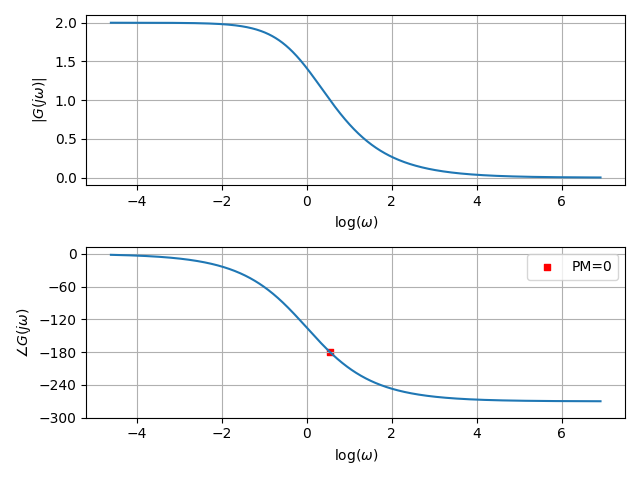
\includegraphics[width=\columnwidth]{2023/IN/50/figs/bode.png}
	\caption{Bode Plot of Transfer Function $G(s)$}
	\label{fig:bode}
\end{figure}

\newpage
\item Consider the second-order linear differential equation
\[x^2\frac{d^2y}{dx^2}+x\frac{dy}{dx}-y=0, \; x\geq 1\]
with the initial conditions \[y(x=1)=6,\; \;\; \frac{dy}{dx}\big{|}_{x=1}=2.\]
Then the value of $y$ at $x=2$ is \rule{2cm}{0.1mm}.\\{\hfill{GATE ME 2023}}\\
\solution
\newpage
\item The transfer function of a measuring instrument is \\
$$G_m(s) = \frac{1.05}{2s+1}exp(-s)$$
At time $t = 0$, a step change of +1 unit is introduced in the input of this instrument.The time taken by the instrument to show an increase of 1 unit in its output is(rounded off to two decimal places).\\ \hfill (GATE CH 2023)
\solution
\item
The laplace transform of $x_1(t)$ = $e^{-t}u(t)$ is $X_1(s)$, where $u(t)$ is the unit step function. The laplace transform of $x_2(t) = e^tu(-t)$ is $X_2(s)$. Which one of the following statements is TRUE?
\begin{enumerate}
    \item The region of convergence of $X_1(s)$ is $Re(s) \geq 0$
    \item The region of convergence of $X_2(s)$ is confined to the left half-plane of s.
    \item The region of convergence of $X_1(s)$ is confined to the right half-plane of s.
    \item the imaginary axis in the s-plane is included in both the region of convergence of $X_1(s)$ and the region of convergence of $X_2(s)$.
\end{enumerate} \hfill(GATE BM 2023)\\
\solution
\iffalse
\let\negmedspace\undefined
\let\negthickspace\undefined
\documentclass[journal,12pt,onecolumn]{IEEEtran}
\usepackage{cite}
\usepackage{amsmath,amssymb,amsfonts,amsthm}
\usepackage{algorithmic}
\usepackage{graphicx}
\usepackage{textcomp}
\usepackage{xcolor}
\usepackage{txfonts}
\usepackage{listings}
\usepackage{enumitem}
\usepackage{mathtools}
\usepackage{gensymb}
\usepackage{comment}
\usepackage[breaklinks=true]{hyperref}
\usepackage{tkz-euclide} 
\usepackage{listings}
\usepackage{gvv}    
\usepackage{enumitem}
\usepackage{amsmath}
\def\inputGnumericTable{}                                 
\usepackage[latin1]{inputenc}                                
\usepackage{color}                                            
\usepackage{array}                                            
\usepackage{longtable}                                       
\usepackage{calc}                                             
\usepackage{multirow}                                         
\usepackage{hhline}                                           
\usepackage{ifthen}                                           
\usepackage{lscape}
\usepackage{tabularx}

\newtheorem{theorem}{Theorem}[section]
\newtheorem{problem}{Problem}
\newtheorem{proposition}{Proposition}[section]
\newtheorem{lemma}{Lemma}[section]
\newtheorem{corollary}[theorem]{Corollary}
\newtheorem{example}{Example}[section]
\newtheorem{definition}[problem]{Definition}
\newcommand{\BEQA}{\begin{eqnarray}}
\newcommand{\EEQA}{\end{eqnarray}}
\newcommand{\define}{\stackrel{\triangle}{=}}
\theoremstyle{remark}
\newtheorem{rem}{Remark}
\begin{document}
\bibliographystyle{IEEEtran}
\vspace{3cm}

\title{GATE-BM-39.2023: }
\author{EE23BTECH11025 - Anantha Krishnan $^{}$% <-this % stops a space
}
\maketitle
\bigskip



\section{question}

The laplace transform of $x_1(t)$ = $e^{-t}u(t)$ is $X_1(s)$, where $u(t)$ is the unit step function. The laplace transform of $x_2(t) = e^tu(-t)$ is $X_2(s)$. Which one of the following statements is TRUE?
\begin{enumerate}
    \item The region of convergence of $X_1(s)$ is $Re(s) \geq 0$
    \item The region of convergence of $X_2(s)$ is confined to the left half-plane of s.
    \item The region of convergence of $X_1(s)$ is confined to the right half-plane of s.
    \item the imaginary axis in the s-plane is included in both the region of convergence of $X_1(s)$ and the region of convergence of $X_2(s)$.
\end{enumerate}
 



\textbf{Solutions :}
\fi
\begin{table}[ht!]
\centering
\begin{tabular}{ |c|c| } 
 \hline
Symbols & Description \\
\hline
 $X_1(s)$ & Laplace transform of $x_1(t)$ \\
 \hline
 $X_2(s)$ & Laplace transform of $x_2(t)$\\
\hline
 $u(t)$ & Unit step function\\
\hline
\end{tabular}
\caption{Parameters, Descriptions}
\label{table:ee25-tab2}
\end{table}




    \begin{enumerate}
        \item 
Laplace transform of $x_1(t)$ is given by :
\begin{align}
    X_1(s) &=  \int_{-\infty}^{\infty} e^{-t}e^{-st}u(t) \,dt
    \end{align}
    Let $s=\sigma+j\omega$ :
\begin{align}
 X_1(s) &= \int_{0}^{\infty}e^{-t\brak{\sigma+1}}e^{-tj\beta} \,dt\\
       &=  \left[\frac{-e^{-t\brak{\sigma+1}}e^{-tj\beta}}{\brak{\sigma+1}+j\beta}\right]_{0}^{\infty}  
       \end{align}
        For $X_1(s)$ to be convergent,$\quad\abs{-e^{-t\brak{\sigma+1}}e^{-tj\beta}}$ must converge $\forall t \epsilon \brak{0,\infty}$, so:
        \begin{align}
\quad\abs{e^{-tj\beta}} = \abs{1}, \forall \beta \epsilon \mathbb{R} \implies Im\brak{s} \epsilon \mathbb{R}\\
\sigma + 1 > 0 \implies  \Re\brak{s}>-1   
        \end{align}
Putting the limits :
       \begin{align}
X_1(s)&= \frac{1}{s+1} , \Re\brak{s} > -1 
\end{align}
\item  
Laplace transform of $x_2(t)$ is given by :
\begin{align}
    X_2(s) &=  \int_{-\infty}^{\infty} e^{t}e^{-st}u(-t) \,dt
        \end{align}
    Let $s=\sigma+j\omega$ :
\begin{align}
    &= \int_{-\infty}^{0}e^{t\brak{1-\sigma}}e^{-tj\beta} \,dt\\
      &=  \left[\frac{e^{t\brak{1-\sigma}}e^{-tj\beta}}{\brak{1-\sigma}-j\beta}\right]_{-\infty}^{0}  
     \end{align}
      For $X_2(s)$ to be convergent,$\quad\abs{e^{t\brak{1-\sigma}}e^{-tj\beta}}$ must converge $\forall t\epsilon\brak{-\infty,0}$, so:
     \begin{align}
\quad\abs{e^{-tj\beta}} = \abs{1}, \forall \beta \epsilon \mathbb{R} \implies Im\brak{s} \epsilon \mathbb{R}\\
1-\sigma > 0 \implies  \Re\brak{s} < 1 
        \end{align}
Putting the limits 
     \begin{align}
            X_2(s)&= \frac{1}{1-s} , \Re\brak{s} < 1
\end{align}
\begin{figure}[h!]
\begin{center}
    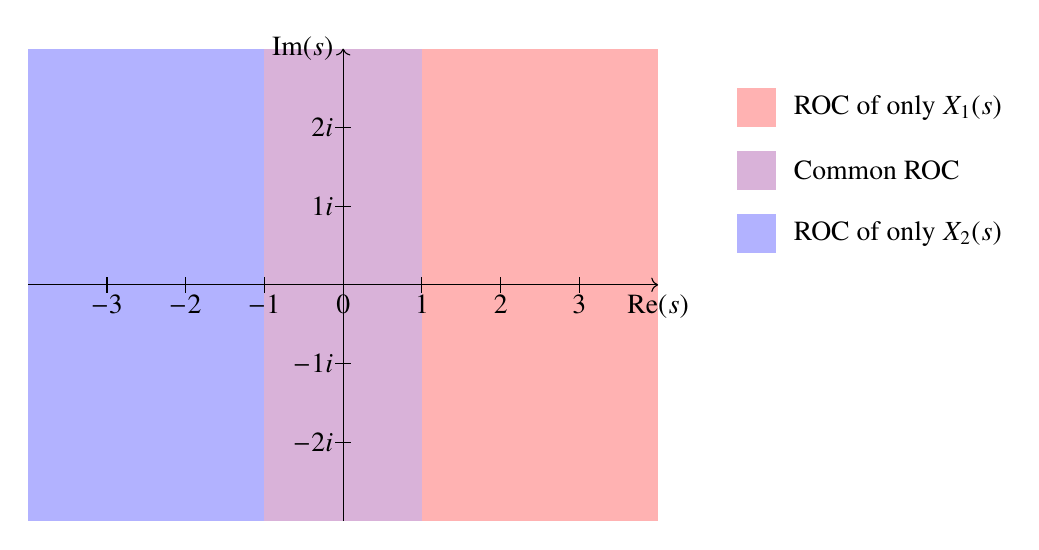
\begin{tikzpicture}
    \fill[red!30] (1,-3) rectangle (4,3);
    \fill[violet!30] (-1,-3) rectangle (1,3);
    \fill[blue!30] (-4,-3) rectangle (-1,3);
    % Axis length
    \draw[->] (-4,0) -- (4,0) node[below] {$\text{Re}(s)$};
    \draw[->] (0,-3) -- (0,3) node[left] {$\text{Im}(s)$};
    % X-axis
    \foreach \x in {-3,-2,-1,0,1,2,3}
        \draw (\x,-0.1) -- (\x,0.1) node[below=3pt] {$\x$};
    % Y-axis
    \foreach \y in {-2,-1,1,2}
        \draw (-0.1,\y) -- (0.1,\y) node[left=3pt] {$\y i$};
    % Legend
    \begin{scope}[shift={(5,2)}]
        \fill[red!30] (0,0) rectangle ++(0.5,0.5);
        \node[right] at (0.6,0.25) {ROC of only $X_1(s)$};
        \fill[violet!30] (0,-0.8) rectangle ++(0.5,0.5);
        \node[right] at (0.6,-0.55) {Common ROC};
        \fill[blue!30] (0,-1.6) rectangle ++(0.5,0.5);
        \node[right] at (0.6,-1.35) {ROC of only $X_2(s)$};
    \end{scope}
\end{tikzpicture}
\caption{Representation of ROCs of $X_1(s)$ and $X_2(s)$} \label{fig:ee23-b1}
\end{center}
\end{figure}


Based on the overlap of regions of convergence of  $X_1(s)$ and $X_2(s)$ from \ref{fig:ee23-b1} , we can conclude that option 4) is correct .  
    \end{enumerate}








\newpage
\item Given that $\frac{dy}{dx}=2x+y$ and $y=1$,when $x=0$ Using Runge-Kutta fourth order method,the value of $y$ at $x=0.2$ is \hfill(GATE 2023 AG 50) \\
\solution

\item The magnitude and phase plots shown in the figure match with the transfer-
function
\begin{figure}[h]
    \centering
    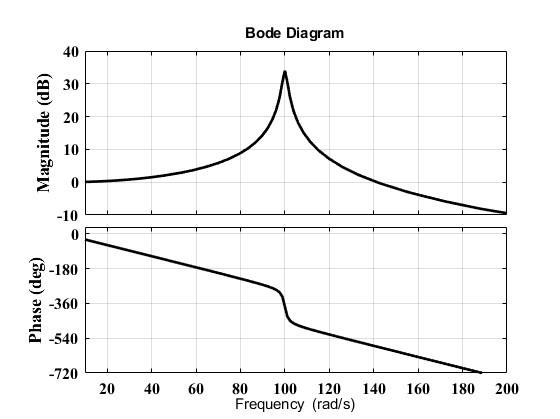
\includegraphics[width=\columnwidth]{2023/IN/43/figs/question.png}
\end{figure}\\
\begin{enumerate}
\item $\frac{10000}{s^2+2s+10000}$\\
\item $\frac{10000}{s^2+2s+10000}e^{-0.05s}$\\
\item $\frac{10000}{s^2+2s+10000}e^{-0.5\times10^{-12}s}$\\
\item $\frac{100}{s^2+2s+100}$
\end{enumerate}
\hfill{(GATE IN 2023)}
\solution

\newpage
\item The Laplace transform of the continuous-time signal $x\brak{t} = e^{-3t}u\brak{t - 5}$ is 
\rule{1cm}{0.15mm}, where $u\brak{t}$ denotes the continuous-time unit step signal.

\begin{enumerate}[label = \Alph*)]
    \item $\frac{e^{-5s}}{s + 3}$, Real$\{s\} > -3$\\
    \item $\frac{e^{-5(s - 3)}}{s - 3}$, Real$\{s\} > 3$\\
    \item $\frac{e^{-5(s + 3)}}{s + 3}$, Real$\{s\} > -3$\\
    \item $\frac{e^{-5(s - 3)}}{s + 3}$, Real$\{s\} > -3$\\
\end{enumerate}
\solution
\iffalse
\let\negmedspace\undefined
\let\negthickspace\undefined
\documentclass[journal,12pt,twocolumn]{IEEEtran}
\usepackage{cite}
\usepackage{amsmath,amssymb,amsfonts,amsthm}
\usepackage{algorithmic}
\usepackage{graphicx}
\usepackage{textcomp}
\usepackage{xcolor}
\usepackage{txfonts}
\usepackage{listings}
\usepackage{enumitem}
\usepackage{mathtools}
\usepackage{gensymb}
\usepackage{comment}
\usepackage[breaklinks=true]{hyperref}
\usepackage{tkz-euclide} 
\usepackage{listings}
\usepackage{gvv}                                        
\def\inputGnumericTable{}                                 
\usepackage[latin1]{inputenc}                                
\usepackage{color}                                            
\usepackage{array}                                            
\usepackage{longtable}                                       
\usepackage{calc}                                             
\usepackage{multirow}                                         
\usepackage{hhline}                                           
\usepackage{ifthen}                                           
\usepackage{lscape}
\usepackage[center]{caption} % center the captions to figure

\newtheorem{theorem}{Theorem}[section]
\newtheorem{problem}{Problem}
\newtheorem{proposition}{Proposition}[section]
\newtheorem{lemma}{Lemma}[section]
\newtheorem{corollary}[theorem]{Corollary}
\newtheorem{example}{Example}[section]
\newtheorem{definition}[problem]{Definition}
\newcommand{\BEQA}{\begin{eqnarray}}
\newcommand{\EEQA}{\end{eqnarray}}
\newcommand{\define}{\stackrel{\triangle}{=}}
\theoremstyle{remark}
\newtheorem{rem}{Remark}
\begin{document}

\newcolumntype{M}[1]{>{\centering\arraybackslash}m{#1}}
\newcolumntype{N}{@{}m{0pt}@{}}

\bibliographystyle{IEEEtran}
\vspace{3cm}

\title{GATE 2023 IN 37Q} 
\author{ee23btech11223 - Soham Prabhakar More% <-this % stops a space
}
\maketitle
\newpage
\bigskip

\renewcommand{\thefigure}{\theenumi}
\renewcommand{\thetable}{\theenumi}

\bibliographystyle{IEEEtran}

\textbf{Question:} The Laplace transform of the continuous-time signal $x\brak{t} = e^{-3t}u\brak{t - 5}$ is 
\rule{1cm}{0.15mm}, where $u\brak{t}$ denotes the continuous-time unit step signal.

\solution
\fi

\begin{table}[ht]
    \begin{tabular}{|c|c|c|} 
    \hline
    \textbf{Variable} & \textbf{Description} & \textbf{Value} \\
    \hline
    $x(t)$ & input function & none \\
    \hline
    $y(t)$ & output function & $\sin(\pi t)$ \\
    \hline
    $H(s)$ & Transfer-function & $\frac{s-\pi}{s+\pi}$ \\
    \hline
\end{tabular}

\end{table}    

\begin{align}
    e^{-3t}u\brak{t} \system{L} \frac{1}{s + 3} \quad \Re\brak{s} > -3 \label{eq:2023.in.37.exp}
\end{align}
Using time shifting,
\begin{align}
    e^{-3(t - 5)}u\brak{t - 5} &\system{L} \frac{e^{-5s}}{s + 3} \\
    e^{-15}e^{-3(t - 5)}u\brak{t - 5} &\system{L} e^{-15}\frac{e^{-5s}}{s + 3} \\
    e^{-3t}u\brak{t - 5} &\system{L} \frac{e^{-5(s + 3)}}{s + 3} \\
    \therefore x\brak{t} &\system{L} \frac{e^{-5(s + 3)}}{s + 3} \quad \Re\brak{s} > -3
\end{align}

\begin{figure}[h!]
    \renewcommand\thefigure{3}
    \centering
    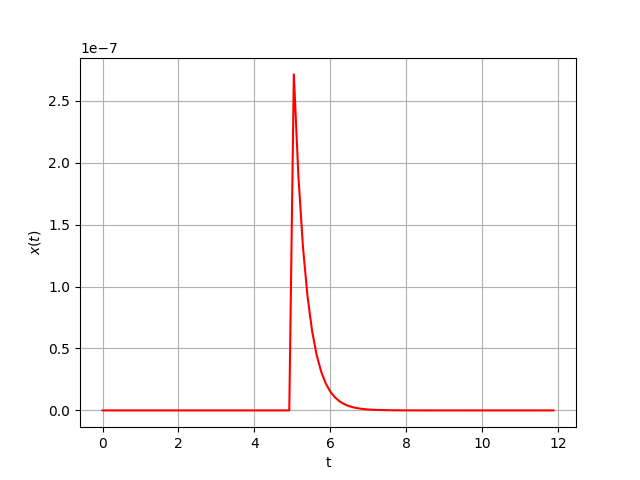
\includegraphics[width=\columnwidth]{figs/x_t.png}
    \caption[short]{Plot of $x\brak{t}$ vs $t$. See \tabref{Table:1}}
    \label{fig:2023.in.37.img1}
\end{figure}

%\end{document}



\newpage
\item The solution $ x(t) ,t \geq 0, $ to the differential equation
$ \ddot{x} = -k\dot{x}  , k > 0 $ with initial conditions $ x(0) = 1 $ and $ x\dot{o}(0) $ = 0 is\\
\solution
\pagebreak
\item  Consider the differential equation
\begin{align}
x^2\frac{d^2y}{dx^2} + 4x\frac{dy}{dx} + 2y = 0 \quad \text{for } x\geq 1 \nonumber
\end{align}
with initial conditions $y=0$ and $\frac{dy}{dx} = 1$ at
$x = 1$. The value of $y$ at $x = 2$ is ?\\

\hfill(GATE AE 54 2023)\\
\solution
\iffalse
\let\negmedspace\undefined
\let\negthickspace\undefined
\documentclass[journal,12pt,twocolumn]{IEEEtran}
\usepackage{cite}
\usepackage{amsmath,amssymb,amsfonts,amsthm}
\usepackage{algorithmic}
\usepackage{graphicx}
\usepackage{textcomp}
\usepackage{xcolor}
\usepackage{txfonts}
\usepackage{listings}
\usepackage{enumitem}
\usepackage{mathtools}
\usepackage{gensymb}
\usepackage{caption}
\usepackage[breaklinks=true]{hyperref}
\usepackage{tkz-euclide} % loads  TikZ and tkz-base
\usepackage{listings}
\usepackage{gvv}
\newtheorem{theorem}{Theorem}[section]
\newtheorem{problem}{Problem}
\newtheorem{proposition}{Proposition}[section]
\newtheorem{lemma}{Lemma}[section]
\newtheorem{corollary}[theorem]{Corollary}
\newtheorem{example}{Example}[section]
\newtheorem{definition}[problem]{Definition}
%\newtheorem{thm}{Theorem}[section] 
%\newtheorem{defn}[thm]{Definition}
%\newtheorem{algorithm}{Algorithm}[section]
%\newtheorem{cor}{Corollary}
\newcommand{\BEQA}{\begin{eqnarray}}
\newcommand{\EEQA}{\end{eqnarray}}
\newcommand{\define}{\stackrel{\triangle}{=}}
\theoremstyle{remark}
\newtheorem{rem}{Remark}

%\bibliographystyle{ieeetr}
\begin{document}
%

\bibliographystyle{IEEEtran}


\vspace{3cm}

\title{
%  \logo{
GATE AE-54(2023)

\large{EE:1205 \brak{Signals  Systems}}

Indian Institute of Technology, Hyderabad
%  }
}
\author{Md Ayaan Ashraf

EE23BTECH11041
}  
\maketitle
\newpage
\bigskip
\renewcommand{\thefigure}{\arabic{figure}}
\renewcommand{\thetable}{\arabic{table}}
%\renewcommand{\theequation}{\theenumi}
\section*{\textit{\textbf{Question}}}
Consider the differential equation
\begin{align}
x^2\frac{d^2y}{dx^2} + 4x\frac{dy}{dx} + 2y = 0 \quad \text{for } x\geq 1 \nonumber
\end{align}
with initial conditions $y=0$ and $\frac{dy}{dx} = 1$ at
$x = 1$. The value of $y$ at $x = 2$ is ?

\hfill {(GATE AE 2023)}
\solution
\fi
\noindent Given : 
\begin{align}
x^2\frac{d^2y}{dx^2} + 4x\frac{dy}{dx} + 2y = 0 \quad \text{for } x\geq 1 \label{eq:given equation}
\end{align}
Using Euler Substitution : 
\begin{align}
x= & e^t \label{eq:x}\\
\frac{dy}{dx}= & e^{-t}\frac{dy}{dt}\label{eq:dy/dx}\\
\frac{d^2y}{dx^2} = & e^{-2t}\frac{d^2y}{dt^2} - e^{-2t}\frac{dy}{dt}\label{eq:d^2y/dx^2}
\end{align}
Substituting equations \eqref{eq:x},\eqref{eq:dy/dx},\eqref{eq:d^2y/dx^2} in equation \eqref{eq:given equation}:
\begin{align}
\frac{d^2y}{dt^2} + 3\frac{dy}{dt} + 2y = 0
\end{align}
Taking Laplace on Both Sides:
\begin{align}
s^2 Y(s) - sy(1)-y'(1) + 3{sY(s) - y(1)} + 2Y(s)= 0\label{eq:laplace}
\end{align}
We know that:
\begin{align}
y(1)=0\label{eq:given 1}\\
y'(1)=1\label{eq:given 2}
\end{align}
Substituting equations \eqref{eq:given 1},\eqref{eq:given 2} in \eqref{eq:laplace}
\begin{align}
s^2Y(s)& + 3sY(s) +2Y(s)= 1\\
\implies Y(s)=&\frac{1}{s^2 + 3s + 2 }\\
\implies Y(s)=&\frac{1}{s+1} - \frac{1}{s+2}
\end{align}
Taking Inverse Laplace:
\begin{align}
y(t) = (e^{-t} - e^{-2t})u(t)
\end{align}
Substituting $x=e^t$:
\begin{align}
y(x)=& e^{-\ln{x}} - e^{-2\ln{x}},\quad x\geq 1 \\
y(x)=& \frac{1}{x} - \frac{1}{x^2},\quad x\geq 1 
\end{align}
\begin{align}
    \therefore y(2) = 0.25
\end{align}
\begin{figure}[ht]
    \centering
    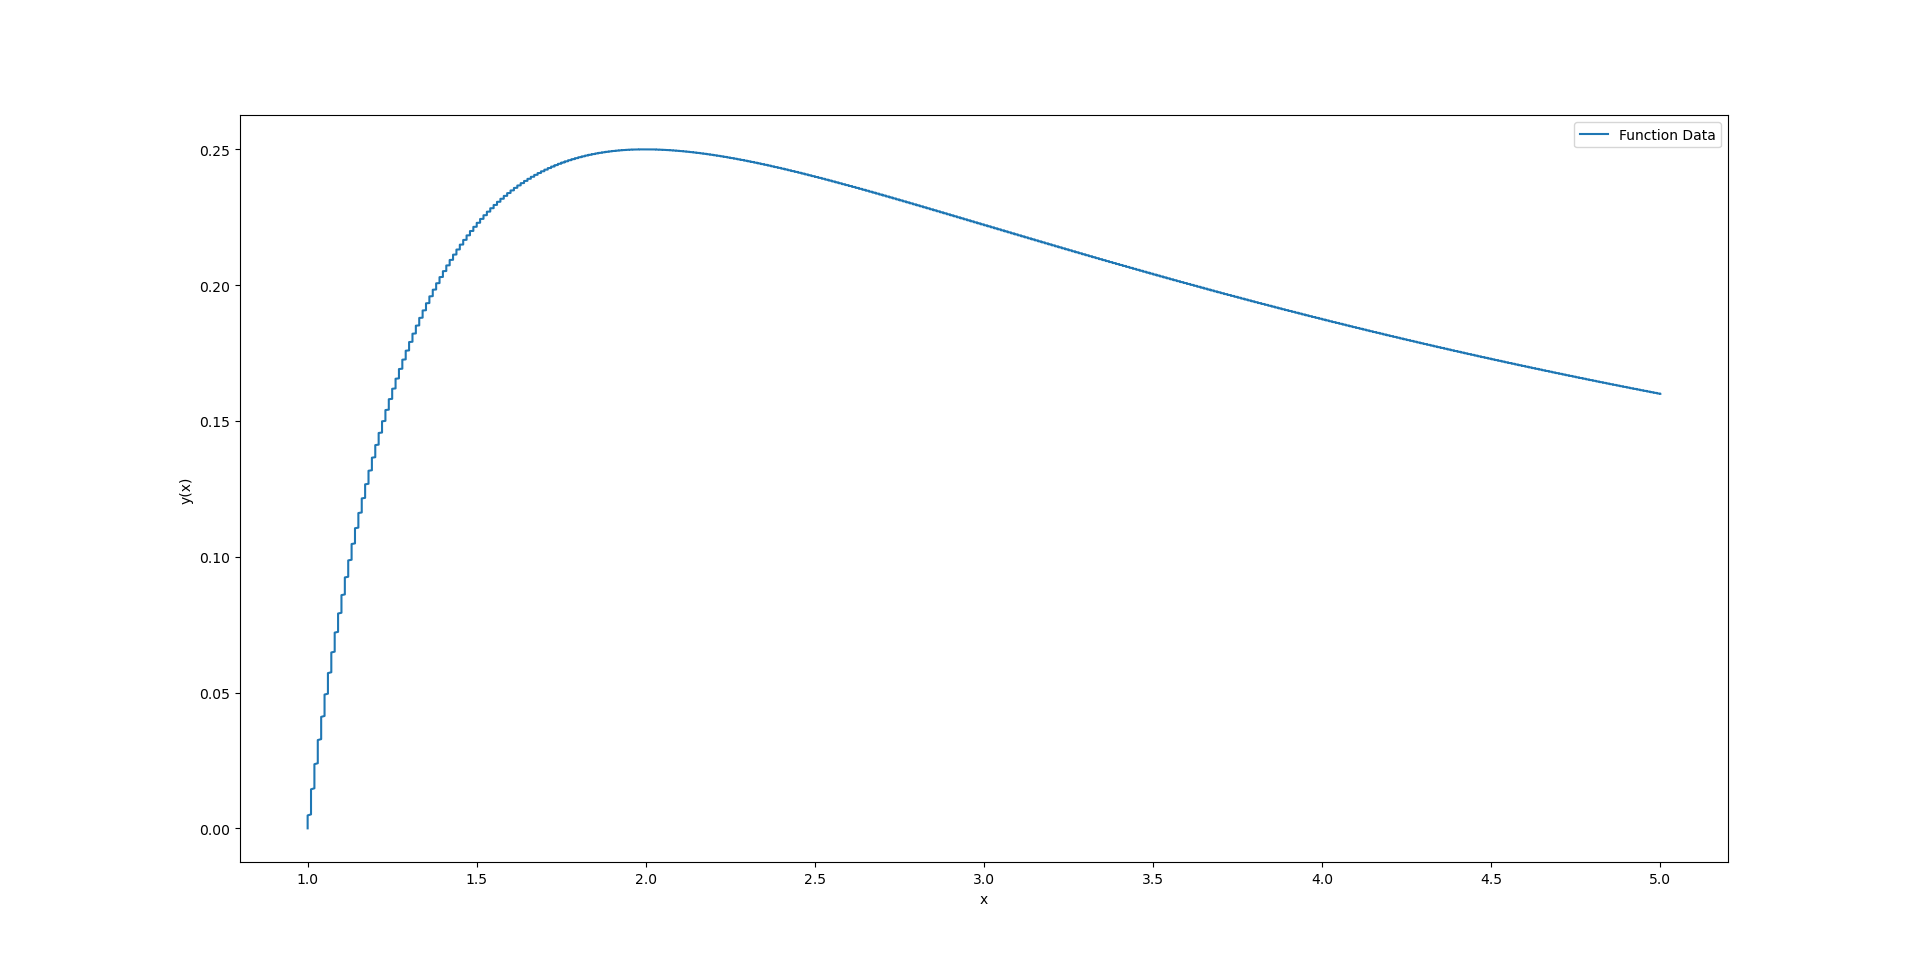
\includegraphics[width=\columnwidth]{2023/AE/54/figs/fig.png}
    \caption{Plot of $y(x)$ $vs$ $x$}
    \label{fig: GATE AE-54(2023)}
\end{figure}

\pagebreak

\item The time-dependent growth of a bacterial population is governed by the equation
\begin{align}
    \frac{dx}{dt}=x\brak{1-\frac{x}{200}}
\end{align}
where $x$ is the population size at time $t$. The initial population size is $x_0=100$
at $x=0$. As $t \rightarrow \infty$, the population size of bacteria asymptotically approaches
\begin{enumerate}[label=(\alph*)]
    \item $150$
    \item $200$
    \item $300$
    \item $500$
\end{enumerate}
\hfill{(GATE BM 2023)}
\solution
\newpage

\item Consider a lead compensator of the form \\
$K(s) = \frac{1 + \frac{s}{a}}{1 + \frac{s}{\beta a}}, \quad \beta > 1, \quad a > 0$\\
The frequency at which this compensator produces maximum phase lead is \(4 \, \text{rad/s}\). At this frequency, the gain amplification provided by the controller, assuming an asymptotic Bode-magnitude plot of \(K(s)\), is \(6 \, \text{dB}\). The values of \(a\) and \(\beta\), respectively, are
\begin{enumerate}
    \item $ 1, 16 $\\
    \item $\ 2, 4 $\\
    \item $ 3, 5 $\\
    \item $ 2.66, 2.25$\\
\end{enumerate}\hfill{(GATE EC 2023)}
\solution
\newpage

\item Second order ordinary differential equation $\frac{d^2y}{dx^2}-\frac{dy}{dx}-2y=0$ has values 
$y=2$ and$\frac{dy}{dx}=1$ at $x=0$.The value of $y$ at $x=1$ is?($round\; off\;\: to\;\: three\;\: decimal\;\: places$)
 \\ \hfill[GATE-ES 2023]\\
 \solution
   \iffalse
\let\negmedspace\undefined
\let\negthickspace\undefined
\documentclass[journal,12pt,twocolumn]{IEEEtran}
\usepackage{xparse}
\usepackage{cite}
\usepackage{amsmath,amssymb,amsfonts,amsthm}
\usepackage{algorithmic}
\usepackage{graphicx}
\usepackage{textcomp}
\usepackage{xcolor}
\usepackage{txfonts}
\usepackage{listings}
\usepackage{enumitem}
\usepackage{mathtools}
\usepackage{gensymb}
\usepackage{comment}
\usepackage[breaklinks=true]{hyperref}
\usepackage{tkz-euclide} 
\usepackage{listings}
\usepackage{gvv}
\def\inputGnumericTable{}                                 
\usepackage[latin1]{inputenc}                                
\usepackage{color}                                            
\usepackage{array}                                            
\usepackage{longtable}                                       
\usepackage{calc}                                             
\usepackage{multirow}                                         
\usepackage{hhline}                                           
\usepackage{ifthen}                                           
\usepackage{lscape}

\newtheorem{theorem}{Theorem}[section]
\newtheorem{problem}{Problem}
\newtheorem{proposition}{Proposition}[section]
\newtheorem{lemma}{Lemma}[section]
\newtheorem{corollary}[theorem]{Corollary}
\newtheorem{example}{Example}[section]
\newtheorem{definition}[problem]{Definition}
\newcommand{\BEQA}{\begin{eqnarray}}
\newcommand{\EEQA}{\end{eqnarray}}
\newcommand{\define}{\stackrel{\triangle}{=}}
\theoremstyle{remark}
\newtheorem{rem}{Remark}
\begin{document}

\bibliographystyle{IEEEtran}
\vspace{3cm}

\title{GATE-ES.47}
\author{EE23BTECH11046 - Poluri Hemanth$^{*}$}
\maketitle
\textbf{Question:}Second order ordinary differential equation $\frac{d^2y}{dx^2}-\frac{dy}{dx}-2y=0$ has values 
$y=2$ and$\frac{dy}{dx}=1$ at $x=0$.The value of $y$ at $x=1$ is?($round\; off\;\: to\;\: three\;\: decimal\;\: places$)
 \\ \hfill[GATE-ES 2023]\\
\textbf{Solution:}\\
\fi
We convert given second order differential equation to s domain using Laplace transform and solve for $Y(s)$ and take inversion to get $y(x)$.
\begin{table}[h!]
    % Change address in github
	%%%%%%%%%%%%%%%%%%%%%%%%%%%%%%%%%%%%%%%%%%%%%%%%%%%%%%%%%%%%%%%%%%%%%%
%%                                                                  %%
%%  This is the header of a LaTeX2e file exported from Gnumeric.    %%
%%                                                                  %%
%%  This file can be compiled as it stands or included in another   %%
%%  LaTeX document. The table is based on the longtable package so  %%
%%  the longtable options (headers, footers...) can be set in the   %%
%%  preamble section below (see PRAMBLE).                           %%
%%                                                                  %%
%%  To include the file in another, the following two lines must be %%
%%  in the including file:                                          %%
%%        \def\inputGnumericTable{}                                 %%
%%  at the beginning of the file and:                               %%
%%        \input{name-of-this-file.tex}                             %%
%%  where the table is to be placed. Note also that the including   %%
%%  file must use the following packages for the table to be        %%
%%  rendered correctly:                                             %%
%%    \usepackage[latin1]{inputenc}                                 %%
%%    \usepackage{color}                                            %%
%%    \usepackage{array}                                            %%
%%    \usepackage{longtable}                                        %%
%%    \usepackage{calc}                                             %%
%%    \usepackage{multirow}                                         %%
%%    \usepackage{hhline}                                           %%
%%    \usepackage{ifthen}                                           %%
%%  optionally (for landscape tables embedded in another document): %%
%%    \usepackage{lscape}                                           %%
%%                                                                  %%
%%%%%%%%%%%%%%%%%%%%%%%%%%%%%%%%%%%%%%%%%%%%%%%%%%%%%%%%%%%%%%%%%%%%%%



%%  This section checks if we are begin input into another file or  %%
%%  the file will be compiled alone. First use a macro taken from   %%
%%  the TeXbook ex 7.7 (suggestion of Han-Wen Nienhuys).            %%
\def\ifundefined#1{\expandafter\ifx\csname#1\endcsname\relax}


%%  Check for the \def token for inputed files. If it is not        %%
%%  defined, the file will be processed as a standalone and the     %%
%%  preamble will be used.                                          %%
\ifundefined{inputGnumericTable}

%%  We must be able to close or not the document at the end.        %%
	\def\gnumericTableEnd{\end{document}}


%%%%%%%%%%%%%%%%%%%%%%%%%%%%%%%%%%%%%%%%%%%%%%%%%%%%%%%%%%%%%%%%%%%%%%
%%                                                                  %%
%%  This is the PREAMBLE. Change these values to get the right      %%
%%  paper size and other niceties.                                  %%
%%                                                                  %%
%%%%%%%%%%%%%%%%%%%%%%%%%%%%%%%%%%%%%%%%%%%%%%%%%%%%%%%%%%%%%%%%%%%%%%

	\documentclass[12pt%
			  %,landscape%
                    ]{report}
       \usepackage[latin1]{inputenc}
       \usepackage{fullpage}
       \usepackage{color}
       \usepackage{array}
       \usepackage{longtable}
       \usepackage{calc}
       \usepackage{multirow}
       \usepackage{hhline}
       \usepackage{ifthen}

	\begin{document}


%%  End of the preamble for the standalone. The next section is for %%
%%  documents which are included into other LaTeX2e files.          %%
\else

%%  We are not a stand alone document. For a regular table, we will %%
%%  have no preamble and only define the closing to mean nothing.   %%
    \def\gnumericTableEnd{}

%%  If we want landscape mode in an embedded document, comment out  %%
%%  the line above and uncomment the two below. The table will      %%
%%  begin on a new page and run in landscape mode.                  %%
%       \def\gnumericTableEnd{\end{landscape}}
%       \begin{landscape}


%%  End f the else clause for this file being \input.              %%
\fi

%%%%%%%%%%%%%%%%%%%%%%%%%%%%%%%%%%%%%%%%%%%%%%%%%%%%%%%%%%%%%%%%%%%%%%
%%                                                                  %%
%%  The rest is the gnumeric table, except for the closing          %%
%%  statement. Changes below will alter the table's appearance.     %%
%%                                                                  %%
%%%%%%%%%%%%%%%%%%%%%%%%%%%%%%%%%%%%%%%%%%%%%%%%%%%%%%%%%%%%%%%%%%%%%%

\providecommand{\gnumericmathit}[1]{#1} 
%%  Uncomment the next line if you would like your numbers to be in %%
%%  italics if they are italizised in the gnumeric table.           %%
%\renewcommand{\gnumericmathit}[1]{\mathit{#1}}
\providecommand{\gnumericPB}[1]%
{\let\gnumericTemp=\\#1\let\\=\gnumericTemp\hspace{0pt}}
 \ifundefined{gnumericTableWidthDefined}
        \newlength{\gnumericTableWidth}
        \newlength{\gnumericTableWidthComplete}
        \newlength{\gnumericMultiRowLength}
        \global\def\gnumericTableWidthDefined{}
 \fi
%% The following setting protects this code from babel shorthands.  %%
 \ifthenelse{\isundefined{\languageshorthands}}{}{\languageshorthands{english}}
%%  The default table format retains the relative column widths of  %%
%%  gnumeric. They can easily be changed to c, r or l. In that case %%
%%  you may want to comment out the next line and uncomment the one %%
%%  thereafter                                                      %%
\providecommand\gnumbox{\makebox[0pt]}
%%\providecommand\gnumbox[1][]{\makebox}

%% to adjust positions in multirow situations                       %%
\setlength{\bigstrutjot}{\jot}
\setlength{\extrarowheight}{\doublerulesep}

%%  The \setlongtables command keeps column widths the same across  %%
%%  pages. Simply comment out next line for varying column widths.  %%
\setlongtables

\setlength\gnumericTableWidth{%
	20pt+%
	40pt+%
	50pt+%	
0pt}
\def\gumericNumCols{3}
\setlength\gnumericTableWidthComplete{\gnumericTableWidth+%
         \tabcolsep*\gumericNumCols*2+\arrayrulewidth*\gumericNumCols}
\ifthenelse{\lengthtest{\gnumericTableWidthComplete > \linewidth}}%
         {\def\gnumericScale{1*\ratio{\linewidth-%
                        \tabcolsep*\gumericNumCols*2-%
                        \arrayrulewidth*\gumericNumCols}%
{\gnumericTableWidth}}}%
{\def\gnumericScale{2}}

%%%%%%%%%%%%%%%%%%%%%%%%%%%%%%%%%%%%%%%%%%%%%%%%%%%%%%%%%%%%%%%%%%%%%%
%%                                                                  %%
%% The following are the widths of the various columns. We are      %%
%% defining them here because then they are easier to change.       %%
%% Depending on the cell formats we may use them more than once.    %%
%%                                                                  %%
%%%%%%%%%%%%%%%%%%%%%%%%%%%%%%%%%%%%%%%%%%%%%%%%%%%%%%%%%%%%%%%%%%%%%%

\ifthenelse{\isundefined{\gnumericColA}}{\newlength{\gnumericColA}}{}\settowidth{\gnumericColA}{\begin{tabular}{@{}p{20pt*\gnumericScale}@{}}x\end{tabular}}
\ifthenelse{\isundefined{\gnumericColB}}{\newlength{\gnumericColB}}{}\settowidth{\gnumericColB}{\begin{tabular}{@{}p{40pt*\gnumericScale}@{}}x\end{tabular}}
\ifthenelse{\isundefined{\gnumericColC}}{\newlength{\gnumericColC}}{}\settowidth{\gnumericColC}{\begin{tabular}{@{}p{50pt*\gnumericScale}@{}}x\end{tabular}}

\begin{tabular}[c]{%
	b{\gnumericColA}%
	b{\gnumericColB}%
	b{\gnumericColC}%
	}

%%%%%%%%%%%%%%%%%%%%%%%%%%%%%%%%%%%%%%%%%%%%%%%%%%%%%%%%%%%%%%%%%%%%%%
%%  The longtable options. (Caption, headers... see Goosens, p.124) %%
%	\caption{The Table Caption.}             \\	%
% \hline	% Across the top of the table.
%%  The rest of these options are table rows which are placed on    %%
%%  the first, last or every page. Use \multicolumn if you want.    %%

%%  Header for the first page.                                      %%
%	\multicolumn{3}{c}{The First Header} \\ \hline 
%	\multicolumn{1}{c}{colTag}	%Column 1
%	&\multicolumn{1}{c}{colTag}	%Column 2
%	&\multicolumn{1}{c}{colTag}	\\ \hline %Last column
%	\endfirsthead

%%  The running header definition.                                  %%
%	\hline
%	\multicolumn{3}{l}{\ldots\small\slshape continued} \\ \hline
%	\multicolumn{1}{c}{colTag}	%Column 1
%	&\multicolumn{1}{c}{colTag}	%Column 2
%	&\multicolumn{1}{c}{colTag}	\\ \hline %Last column
%	\endhead

%%  The running footer definition.                                  %%
%	\hline
%	\multicolumn{3}{r}{\small\slshape continued\ldots} \\
%	\endfoot

%%  The ending footer definition.                                   %%
%	\multicolumn{3}{c}{That's all folks} \\ \hline 
%	\endlastfoot
%%%%%%%%%%%%%%%%%%%%%%%%%%%%%%%%%%%%%%%%%%%%%%%%%%%%%%%%%%%%%%%%%%%%%%
\hhline{|-|-|-}
	\multicolumn{1}{|p{\gnumericColA}|}%
	{\gnumericPB{\centering}\gnumbox{\textbf{Symbol}}}
	&\multicolumn{1}{p{\gnumericColB}|}%
	{\gnumericPB{\centering}\gnumbox{\textbf{Values}}}
	&\multicolumn{1}{p{\gnumericColC}|}%
	{\gnumericPB{\centering}\gnumbox{\textbf{Description}}}

\\
\hhline{|---|}
	\multicolumn{1}{|p{\gnumericColA}|}%
	{\gnumericPB{\centering}\gnumbox{$Y(s)$}}
	&\multicolumn{1}{p{\gnumericColB}|}%
	{\gnumericPB{\centering}\gnumbox{$\frac{2s-1}{s^2-s-2}$}}
	&\multicolumn{1}{p{\gnumericColC}|}%
	{\gnumericPB{\centering}\gnumbox{$y$ in s domain}}

\\
\hhline{|---|}
        \multicolumn{1}{|p{\gnumericColA}|}%
	{\gnumericPB{\centering}\gnumbox{$y(x)$}}             
        &\multicolumn{1}{p{\gnumericColB}|}%
	{\gnumericPB{\centering}\gnumbox{$e^{2x}+e^{-x}$}}  
        &\multicolumn{1}{p{\gnumericColC}|}%
	{\gnumericPB{\centering}\gnumbox{$y$ in x domain}}

\\
\hhline{|---|}
        \multicolumn{1}{|p{\gnumericColA}|}%
        {\gnumericPB{\centering}\gnumbox{$y(0)$}}             
        &\multicolumn{1}{p{\gnumericColB}|}%
        {\gnumericPB{\centering}\gnumbox{2}}  
        &\multicolumn{1}{p{\gnumericColC}|}%
        {\gnumericPB{\centering}\gnumbox{$y$ at $x=0$}}
\\
\hhline{|---|}
        \multicolumn{1}{|p{\gnumericColA}|}%
        {\gnumericPB{\centering}\gnumbox{$y'(0)$}}             
        &\multicolumn{1}{p{\gnumericColB}|}%
        {\gnumericPB{\centering}\gnumbox{1}}  
        &\multicolumn{1}{p{\gnumericColC}|}%
	{\gnumericPB{\centering}\gnumbox{$y'(x)$ at $x=0$}}

\\
\hhline{|---|}
        \multicolumn{1}{|p{\gnumericColA}|}%
	{\gnumericPB{\centering}\gnumbox{$u(x)$}}             
        &\multicolumn{1}{p{\gnumericColB}|}%
	{\gnumericPB{\centering}\gnumbox{$=\begin{cases}
        1 & \text{if } x \geq 0\\
        0 &  o.w
    \end{cases}$}}  
        &\multicolumn{1}{p{\gnumericColC}|}%
        {\gnumericPB{\centering}\gnumbox{unit step function}}
\\
\hhline{|-|-|-|}
\end{tabular}

\ifthenelse{\isundefined{\languageshorthands}}{}{\languageshorthands{\languagename}}
\gnumericTableEnd

        \caption{Parameters}
        \label{tab:es.47}
\end{table}


\begin{align}
    \frac{d^2y}{dx^2}-\frac{dy}{dx}-2y&\Large\xleftrightarrow{\mathcal{L}}s^2Y(s)-sy(0)-y'(0)-sY(s)+y(0)-2Y(s)\\
	Y(s)\left(s^2-s-2\right)&=2s-1\\
    \Rightarrow Y(s)&=\frac{2s-1}{s^2-s-2}\\
    \Rightarrow Y(s)&=\frac{1}{s-2}+\frac{1}{s+1}
\end{align}
For inversion of $Y(s)$ in partial fractions-
\begin{align}
	&\frac{b}{s+a}\Large\xleftrightarrow{\mathcal{L}^{-1}}be^{-ax}u(x)\label{inv}
\end{align}
Where b, a are real numbers, we invert $Y(s)$ to get $y(x)$:-\\
From \eqref{inv}
\begin{align}
	&Y(s)\Large\xleftrightarrow{\mathcal{L}^{-1}} y(x)u(x)
\end{align}
\begin{align}
	y(x)&=\left(e^{2x}+e^{-x}\right)u(x)\\
   \Rightarrow y(1)&=7.757
\end{align}\\
\begin{figure}[h!]
    \centering
    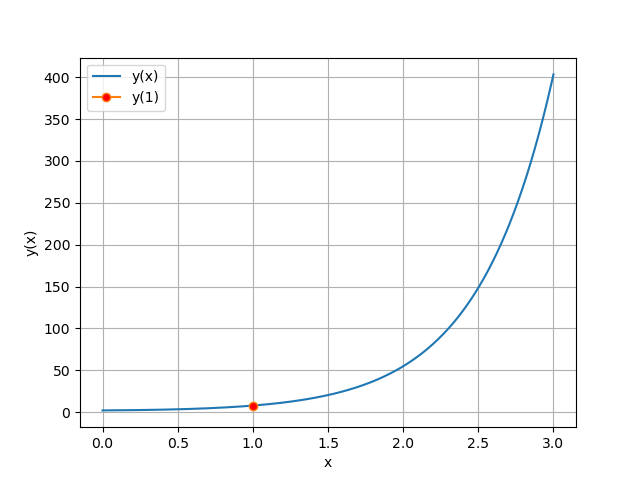
\includegraphics[width=1\linewidth]{2023/ES/47/figures/gate.png}
	\caption{Plot of y(x)}
    \label{fig:enter-label}
\end{figure}






%\end{document}

 \newpage

 \item A continuous-time system that is initially at rest is described by,	
	\begin{center}
		$\dfrac{dy(t)}{dt} + 3y(t) = 2x(t)$
	\end{center}
where $x(t)$ is the input voltage and $y(t)$ is the output voltage.\\ 
The impulse response of the system is?
\hfill(GATE 2023 EE)
\solution
\newpage

\item Consider the equation $\frac{dy}{dx}+ay=\sin{\omega x}$,where $a$ and $\omega$ are constants.Given $y=1$ at $x=0$, correct all the correct statement(s) from the following as $x\to \infty$.
\begin{enumerate}

  \item[(A)]  $y \to 0$ if $a \neq 0$ \\ 
  \item[(B)]  $y \to 1$ if $a = 0$\\
  \item[(C)]  $y \to Aexp(|a|x)$ if $a < 0$; A is constant\\
  \item[(D)]  $y \to B \sin(\omega x+C)$ if $a>0$; B and C are constants\\
\end{enumerate}
\hfill(GATE AE 2023)
\solution
\newpage


\item \textbf{Question }:
The position $x(t)$ of a particle, at constant $\omega$, is described by the equation
\begin{align}
\frac{{d^2x}}{{dt^2}} = -\omega^2 x.
\end{align}
The initial conditions are $x(t=0)=1$ and $\frac{{dx}}{{dt}}\bigg|_{t=0}=0$. 
The position of the particle at $t=\frac{{3\pi}}{{\omega}}$ is \underline{\hspace{2cm}} (in integer).
\hfill{(GATE CH 2023)}
\solution
\newpage

\item \textbf{Question}:The initial value problem
$\frac{dy}{dt}+2y=0, y(0)=1 $
is solved numerically using the forward Euler's method with a constant and positive time step of $\delta $.\\
Let $y_n$ represent the numerical solution obtained after $n$ steps. The condition $\abs{y_{n+1}} \leq \abs{y_n}$is satisfied if and only if $\delta$ does not exceed \\
\hfill{(GATE ME 2023)}
\solution
\newpage

\item In the context of signals and systems, determine the phase cross-over frequency of the open-loop transfer function
\[
G(s) = \frac{k \cdot s \cdot (1+sT_1) \cdot (1+sT_2)}{s}
\]
with positive constants $k, T_1, T_2$ are positive constants.The phase crossover fequency,in rad/s,is
\begin{enumerate}
  \item[(a)] $\frac{1}{\sqrt{T_1 T_2}}$
  \item[(b)] $\frac{1}{T_1 T_2}$
  \item[(c)] $\frac{1}{T_1\sqrt{T_2}}$
  \item[(d)] $\frac{1}{\sqrt{T_2}T_1}$
\end{enumerate}
\hfill{(GATE EC 2023)}
\solution
\newpage

\item Which one of the options given is the inverse Laplace transform of $\frac{1}{s^3-s}$?\\
$u(t)$ denotes the unit-step function.
\begin{enumerate}[label=(\Alph*)]
\item $\left(-1+\frac{1}{2}e^{-t}+\frac{1}{2}e^t\right)u(t)$\\
\item $\left(\frac{1}{3}e^{-t}-e^t\right)u(t)$\\
\item $\left(-1+\frac{1}{2}e^{-(t-1)}+\frac{1}{2}e^{(t-1)}\right)u(t-1)$\\
\item $\left(-1-\frac{1}{2}e^{-(t-1)}-\frac{1}{2}e^{(t-1)}\right)u(t-1)$\\
\end{enumerate}
\hfill(GATE ME 2023)\\
\solution
\let\negmedspace\undefined
\let\negthickspace\undefined
\documentclass[journal,12pt,onecolumn]{IEEEtran}
\usepackage{cite}
\usepackage{amsmath,amssymb,amsfonts,amsthm}
\usepackage{algorithmic}
\usepackage{graphicx}
\usepackage{textcomp}
\usepackage{xcolor}
\usepackage{txfonts}
\usepackage{listings}
\usepackage{enumitem}
\usepackage{mathtools}
\usepackage{gensymb}
\usepackage{comment}
\usepackage[breaklinks=true]{hyperref}
\usepackage{tkz-euclide} % loads  TikZ and tkz-base
\usepackage{listings}
\usepackage[latin1]{inputenc}                                
\usepackage{color}                                            
\usepackage{array}                                            
\usepackage{longtable}                                       
\usepackage{calc}                                             
\usepackage{multirow}                                         
\usepackage{hhline}                                           
\usepackage{ifthen}                                           
\usepackage{lscape}
\usepackage{caption}
\usepackage{subcaption}
\usepackage{float}


\newtheorem{theorem}{Theorem}[section]
\newtheorem{problem}{Problem}
\newtheorem{proposition}{Proposition}[section]
\newtheorem{lemma}{Lemma}[section]
\newtheorem{corollary}[theorem]{Corollary}
\newtheorem{example}{Example}[section]
\newtheorem{definition}[problem]{Definition}
%\newtheorem{thm}{Theorem}[section] 
%\newtheorem{defn}[thm]{Definition}
%\newtheorem{algorithm}{Algorithm}[section]
%\newtheorem{cor}{Corollary}
\newcommand{\BEQA}{\begin{eqnarray}}
\newcommand{\EEQA}{\end{eqnarray}}
\newcommand{\define}{\stackrel{\triangle}{=}}
\theoremstyle{remark}
\newtheorem{rem}{Remark}
%\bibliographystyle{ieeetr}

\begin{document}

%
\providecommand{\pr}[1]{\ensuremath{\Pr\left(#1\right)}}
\providecommand{\prt}[2]{\ensuremath{p_{#1}^{\left(#2\right)} }}        % own macro for this question
\providecommand{\qfunc}[1]{\ensuremath{Q\left(#1\right)}}
\providecommand{\sbrak}[1]{\ensuremath{{}\left[#1\right]}}
\providecommand{\lsbrak}[1]{\ensuremath{{}\left[#1\right.}}
\providecommand{\rsbrak}[1]{\ensuremath{{}\left.#1\right]}}
\providecommand{\brak}[1]{\ensuremath{\left(#1\right)}}
\providecommand{\lbrak}[1]{\ensuremath{\left(#1\right.}}
\providecommand{\rbrak}[1]{\ensuremath{\left.#1\right)}}
\providecommand{\cbrak}[1]{\ensuremath{\left\{#1\right\}}}
\providecommand{\lcbrak}[1]{\ensuremath{\left\{#1\right.}}
\providecommand{\rcbrak}[1]{\ensuremath{\left.#1\right\}}}
\newcommand{\sgn}{\mathop{\mathrm{sgn}}}
\providecommand{\abs}[1]{\left\vert#1\right\vert}
\providecommand{\res}[1]{\Res\displaylimits_{#1}} 
\providecommand{\norm}[1]{\left\lVert#1\right\rVert}
%\providecommand{\norm}[1]{\lVert#1\rVert}
\providecommand{\mtx}[1]{\mathbf{#1}}
\providecommand{\mean}[1]{E\left[ #1 \right]}
\providecommand{\cond}[2]{#1\middle|#2}
\providecommand{\fourier}{\overset{\mathcal{F}}{ \rightleftharpoons}}
\newenvironment{amatrix}[1]{%
  \left(\begin{array}{@{}*{#1}{c}|c@{}}
}{%
  \end{array}\right)
}
%\providecommand{\hilbert}{\overset{\mathcal{H}}{ \rightleftharpoons}}
%\providecommand{\system}{\overset{\mathcal{H}}{ \longleftrightarrow}}
        %\newcommand{\solution}[2]{\textbf{Solution:}{#1}}
\newcommand{\solution}{\noindent \textbf{Solution: }}
\newcommand{\cosec}{\,\text{cosec}\,}
\providecommand{\dec}[2]{\ensuremath{\overset{#1}{\underset{#2}{\gtrless}}}}
\newcommand{\myvec}[1]{\ensuremath{\begin{pmatrix}#1\end{pmatrix}}}
\newcommand{\mydet}[1]{\ensuremath{\begin{vmatrix}#1\end{vmatrix}}}
\newcommand{\myaugvec}[2]{\ensuremath{\begin{amatrix}{#1}#2\end{amatrix}}}
\providecommand{\rank}{\text{rank}}
\providecommand{\pr}[1]{\ensuremath{\Pr\left(#1\right)}}
\providecommand{\qfunc}[1]{\ensuremath{Q\left(#1\right)}}
        \newcommand*{\permcomb}[4][0mu]{{{}^{#3}\mkern#1#2_{#4}}}
\newcommand*{\perm}[1][-3mu]{\permcomb[#1]{P}}
\newcommand*{\comb}[1][-1mu]{\permcomb[#1]{C}}
\providecommand{\qfunc}[1]{\ensuremath{Q\left(#1\right)}}
\providecommand{\gauss}[2]{\mathcal{N}\ensuremath{\left(#1,#2\right)}}
\providecommand{\diff}[2]{\ensuremath{\frac{d{#1}}{d{#2}}}}
\providecommand{\myceil}[1]{\left \lceil #1 \right \rceil }
\newcommand\figref{Fig.~\ref}
\newcommand\tabref{Table~\ref}
\newcommand{\sinc}{\,\text{sinc}\,}
\newcommand{\rect}{\,\text{rect}\,}
%%
%       %\newcommand{\solution}[2]{\textbf{Solution:}{#1}}
%\newcommand{\solution}{\noindent \textbf{Solution: }}
%\newcommand{\cosec}{\,\text{cosec}\,}
%\numberwithin{equation}{section}
%\numberwithin{equation}{subsection}
%\numberwithin{problem}{section}
%\numberwithin{definition}{section}
%\makeatletter
%\@addtoreset{figure}{problem}
%\makeatother

%\let\StandardTheFigure\thefigure
\let\vec\mathbf

\bibliographystyle{IEEEtran}

\vspace{3cm}
\title{Assignment}
\author{EE23BTECH11001 - Aashna Sahu}
\maketitle
\bigskip

\renewcommand{\thefigure}{\theenumi}
\renewcommand{\thetable}{\theenumi}
%\renewcommand{\theequation}{\theenumi}
Q:Which one of the options given is the inverse Laplace transform of $\frac{1}{s^3-s}$?\\
$u(t)$ denotes the unit-step function.
\begin{enumerate}[label=(\Alph*)]
\item $\left(-1+\frac{1}{2}e^{-t}+\frac{1}{2}e^t\right)u(t)$\\
\item $\left(\frac{1}{3}e^{-t}-e^t\right)u(t)$\\
\item $\left(-1+\frac{1}{2}e^{-(t-1)}+\frac{1}{2}e^{(t-1)}\right)u(t-1)$\\
\item $\left(-1-\frac{1}{2}e^{-(t-1)}-\frac{1}{2}e^{(t-1)}\right)u(t-1)$\\
\end{enumerate}
\hfill(GATE ME 2023)

\solution
\\
Using partial fraction,\\
\begin{align}
\frac{1}{s^3-s}=\frac{A}{s}+\frac{B}{s+1}+\frac{C}{s-1}
\end{align}
On Solving,
\begin{align}
\implies A=-1\quad B=\frac{1}{2} \quad C=\frac{1}{2}\\
X(s)=\frac{-1}{s}+\frac{1}{2(s+1)}+\frac{1}{2(s-1)}\\
\text{As} \quad e^{-at}u(t) \xrightarrow{\mathcal{L}} \frac{1}{s+a}\quad \Re(s)>-a\\
\text{And} \quad -e^{-at}u(-t) \xrightarrow{\mathcal{L}} \frac{1}{s+a}\quad \Re(s)<-a
\end{align}
Now,
\begin{align}
\mathcal{L}^{-1}(X(s))=x(t)
\end{align}

There are 4 cases possible,
\begin{align}
x(t)=
\begin{cases}
        \left(1-\frac{1}{2}e^{-t}-\frac{1}{2}e^t\right)u(-t) & \Re(s)<-1 \\
        \\
        -1u(-t)+\frac{1}{2}e^{-t}u(t)-\frac{1}{2}e^tu(-t) & \Re(s)\in(-1,0)\\
        \\
        -u(t)+\frac{1}{2}e^{-t}u(t)-\frac{1}{2}e^tu(-t) & \Re(s)\in(0,1)\\
        \\
        \left(-1+\frac{1}{2}e^{-t}+\frac{1}{2}e^t\right)u(t) & \Re(s)>1
\end{cases}
\end{align}\\
 
Thus the correct option is (A) $\left(-1+\frac{1}{2}e^{-t}+\frac{1}{2}e^t\right)u(t)$ for $\Re(s)>1$

\begin{figure}[H]
  \centering
  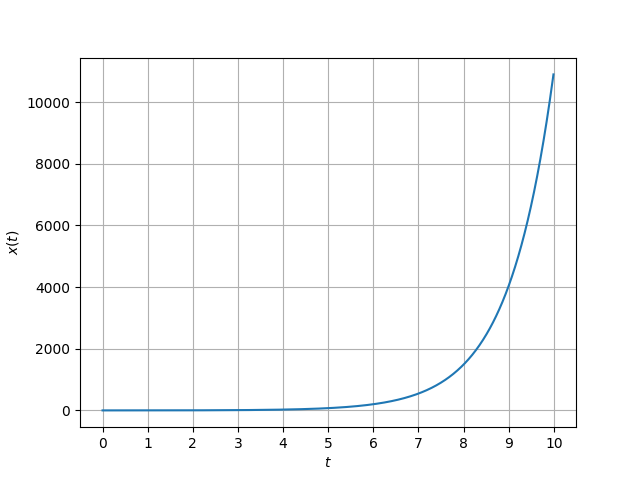
\includegraphics[width=1.0\columnwidth]{figs/plot1.png}
  \caption{Plot for x(t)=$\left(-1+\frac{1}{2}e^{-t}+\frac{1}{2}e^t\right)u(t)$}
  \label{fig:fig1}
\end{figure}
\end{document}

\newpage

\item The state equation of a second order system is \\
$ \dot{{x}}(t) = A{x}(t)$, \quad ${x}(0)$ is the initial condition. \\
Suppose $\lambda_1$ and $\lambda_2$ are two distinct eigenvalues of $A$, and $\nu_1$ and $\nu_2$ are the corresponding eigenvectors. For constants $\alpha_1$ and $\alpha_2$, the solution, ${x}(t)$, of the state equation is \\
\begin{enumerate}[label=(\Alph*)]
\item $\sum_{i=1}^{2} \alpha_ie^{\lambda_it}\bf{\nu}_i$
\item $\sum_{i=1}^{2} \alpha_ie^{2\lambda_it}\bf{\nu}_i$
\item $\sum_{i=1}^{2} \alpha_ie^{3\lambda_it}\bf{\nu}_i$
\item $\sum_{i=1}^{2} \alpha_ie^{4\lambda_it}\bf{\nu}_i$
\end{enumerate}
\hfill{GATE EC 2023}\\
\solution
\iffalse
\let\negmedspace\undefined
\let\negthickspace\undefined
\documentclass[journal,12pt,onecolumn]{IEEEtran}
\usepackage{cite}
\usepackage{amsmath,amssymb,amsfonts,amsthm}
%\usepackage{algorithmic}
\usepackage{graphicx}
\usepackage{textcomp}
\usepackage{array}
\usepackage{xcolor}
\usepackage{txfonts}
\usepackage{listings}
\usepackage{enumitem}
\usepackage{mathtools}
\usepackage{gensymb}
\usepackage[breaklinks=true]{hyperref}
\usepackage{tkz-euclide} % loads  TikZ and tkz-base
\usepackage{listings}
\usepackage{float}
\usepackage{bm}



\newtheorem{theorem}{Theorem}[section]
\newtheorem{problem}{Problem}
\newtheorem{proposition}{Proposition}[section]
\newtheorem{lemma}{Lemma}[section]
\newtheorem{corollary}[theorem]{Corollary}
\newtheorem{example}{Example}[section]
\newtheorem{definition}[problem]{Definition}
%\newtheorem{thm}{Theorem}[section] 
%\newtheorem{defn}[thm]{Definition}
%\newtheorem{algorithm}{Algorithm}[section]
%\newtheorem{cor}{Corollary}
\newcommand{\BEQA}{\begin{eqnarray}}
\newcommand{\EEQA}{\end{eqnarray}}
\newcommand{\define}{\stackrel{\triangle}{=}}
\theoremstyle{remark}
\newtheorem{rem}{Remark}
%\bibliographystyle{ieeetr}
\begin{document}
%
\providecommand{\pr}[1]{\ensuremath{\Pr\left(#1\right)}}
\providecommand{\prt}[2]{\ensuremath{p_{#1}^{\left(#2\right)} }}        % own macro for this question
\providecommand{\qfunc}[1]{\ensuremath{Q\left(#1\right)}}
\providecommand{\sbrak}[1]{\ensuremath{{}\left[#1\right]}}
\providecommand{\lsbrak}[1]{\ensuremath{{}\left[#1\right.}}
\providecommand{\rsbrak}[1]{\ensuremath{{}\left.#1\right]}}
\providecommand{\brak}[1]{\ensuremath{\left(#1\right)}}
\providecommand{\lbrak}[1]{\ensuremath{\left(#1\right.}}
\providecommand{\rbrak}[1]{\ensuremath{\left.#1\right)}}
\providecommand{\cbrak}[1]{\ensuremath{\left\{#1\right\}}}
\providecommand{\lcbrak}[1]{\ensuremath{\left\{#1\right.}}
\providecommand{\rcbrak}[1]{\ensuremath{\left.#1\right\}}}
\newcommand{\sgn}{\mathop{\mathrm{sgn}}}
\providecommand{\abs}[1]{\left\vert#1\right\vert}
\providecommand{\res}[1]{\Res\displaylimits_{#1}} 
\providecommand{\norm}[1]{\left\lVert#1\right\rVert}
%\providecommand{\norm}[1]{\lVert#1\rVert}
\providecommand{\mtx}[1]{\mathbf{#1}}
\providecommand{\mean}[1]{E\left[ #1 \right]}
\providecommand{\cond}[2]{#1\middle|#2}
\providecommand{\fourier}{\overset{\mathcal{F}}{ \rightleftharpoons}}
\newenvironment{amatrix}[1]{%
  \left(\begin{array}{@{}*{#1}{c}|c@{}}
}{%
  \end{array}\right)
}
%\providecommand{\hilbert}{\overset{\mathcal{H}}{ \rightleftharpoons}}
%\providecommand{\system}{\overset{\mathcal{H}}{ \longleftrightarrow}}
	%\newcommand{\solution}[2]{\textbf{Solution:}{#1}}
\newcommand{\solution}{\noindent \textbf{Solution: }}
\newcommand{\cosec}{\,\text{cosec}\,}
\providecommand{\dec}[2]{\ensuremath{\overset{#1}{\underset{#2}{\gtrless}}}}
\newcommand{\myvec}[1]{\ensuremath{\begin{pmatrix}#1\end{pmatrix}}}
\newcommand{\mydet}[1]{\ensuremath{\begin{vmatrix}#1\end{vmatrix}}}
\newcommand{\myaugvec}[2]{\ensuremath{\begin{amatrix}{#1}#2\end{amatrix}}}
\providecommand{\rank}{\text{rank}}
\providecommand{\pr}[1]{\ensuremath{\Pr\left(#1\right)}}
\providecommand{\qfunc}[1]{\ensuremath{Q\left(#1\right)}}
	\newcommand*{\permcomb}[4][0mu]{{{}^{#3}\mkern#1#2_{#4}}}
\newcommand*{\perm}[1][-3mu]{\permcomb[#1]{P}}
\newcommand*{\comb}[1][-1mu]{\permcomb[#1]{C}}
\providecommand{\qfunc}[1]{\ensuremath{Q\left(#1\right)}}
\providecommand{\gauss}[2]{\mathcal{N}\ensuremath{\left(#1,#2\right)}}
\providecommand{\diff}[2]{\ensuremath{\frac{d{#1}}{d{#2}}}}
\providecommand{\myceil}[1]{\left \lceil #1 \right \rceil }
\newcommand\figref{Fig.~\ref}
\newcommand\tabref{Table~\ref}
\newcommand{\sinc}{\,\text{sinc}\,}
\newcommand{\rect}{\,\text{rect}\,}
%%
%	%\newcommand{\solution}[2]{\textbf{Solution:}{#1}}
%\newcommand{\solution}{\noindent \textbf{Solution: }}
%\newcommand{\cosec}{\,\text{cosec}\,}
%\numberwithin{equation}{section}
%\numberwithin{equation}{subsection}
%\numberwithin{problem}{section}
%\numberwithin{definition}{section}
%\makeatletter
%\@addtoreset{figure}{problem}
%\makeatother

%\let\StandardTheFigure\thefigure
\let\vec\mathbf

\bibliographystyle{IEEEtran}





\bigskip

%\renewcommand{\thefigure}{\theenumi}
%\renewcommand{\thetable}{\theenumi}
%\renewcommand{\theequation}{\theenumi}

Q: The state equation of a second order system is \\
$ \dot{{x}}(t) = A{x}(t)$, \quad ${x}(0)$ is the initial condition. \\
Suppose $\lambda_1$ and $\lambda_2$ are two distinct eigenvalues of $A$, and $\nu_1$ and $\nu_2$ are the corresponding eigenvectors. For constants $\alpha_1$ and $\alpha_2$, the solution, ${x}(t)$, of the state equation is \\
\begin{enumerate}[label=(\Alph*)]
\item $\sum_{i=1}^{2} \alpha_ie^{\lambda_it}\bf{\nu}_i$
\item $\sum_{i=1}^{2} \alpha_ie^{2\lambda_it}\bf{\nu}_i$
\item $\sum_{i=1}^{2} \alpha_ie^{3\lambda_it}\bf{\nu}_i$
\item $\sum_{i=1}^{2} \alpha_ie^{4\lambda_it}\bf{\nu}_i$
\end{enumerate}
\hfill{GATE EC 2023}


\solution \\
\fi
%$ \dot{\bm{x}}(t) = A\bm{x}(t)$ \\
%If $\lambda$ is the eigen value of matrix A then $ \dot{\bm{x}}(t) = \lambda\bm{x}(t)$ \\
%As there are 2 eigen values $\lambda_1$ and $\lambda_2$ of matrix A, the solution of state equation will be, \\
%$x(t) = \sum_{i=1}^{2} \alpha_ie^{\lambda_it}\bf{\nu}_i$ \\
%Hence, the correct option is (A). \\
\begin{table}[!ht]
    \centering
        \begin{tabular}{|c|c|c|} 
      \hline
\textbf{Variable}& \textbf{Description}& \textbf{Value}\\\hline
	 ${x}(t)$ & state variable & - \\\hline
         $\dot{{x}}(t)$ & derivative of x(t) w.r.t t & $\frac{d{x}(t)}{dt}$\\\hline  
         A & $2x2$ matrix & -\\\hline
         $\lambda _i$ for $i = 1, 2$ & eigen values of A & - \\\hline
         $v_i$ for $i = 1, 2$ & eigen vectors of A & - \\\hline
         $\alpha _i$ for $i = 1, 2$ & component of $x(t)$ along $v_i$ & - \\\hline
    \end{tabular}

    \caption{input parameters}
    \label{tab:gate23EC43.1}
\end{table}

\textbf{Theories and Proofs:} \\
\begin{align}
A\vec{y} &= \lambda \vec{y} 
\end{align}
Eigen values of inverse of a matrix is reciprocal of eigen value of the given matrix\\
\begin{align}
A^{-1}A\vec{y} &= A^{-1}\lambda \vec{y} \\ \implies
\vec{y} &= \lambda A^{-1}\vec{y}  \\ \implies
A^{-1} \vec{y} &= \frac{1}{\lambda}\vec{y} \label{eq:gate23EC43.1}
\end{align}
Eigen value of a matrix shifts by the same amount as that of the matrix.\\
\begin{align}
(A - \sigma I)\vec{y} &= A\vec{y} - \sigma I\vec{y} \\
&= \lambda \vec{y} - \sigma \vec{y} \\
&= (\lambda - \sigma) \vec{y} \label{eq:gate23EC43.2}
\end{align}
\textbf{Sol:} \\
Using Laplace transform: \\
Given Equation:
\begin{align}
\dot{{x}}(t) &= A{x}(t) \\
\frac{d{x}(t)}{dt} &= A{x}(t) 
\end{align}
Taking Laplace Transform:
\begin{align}
\mathcal{L}\brak{\frac{d{x}(t)}{dt}} &= \mathcal{L}\brak{A{x}(t)} \\
sX(s) - {x}(0) &= AX(s) \\
(sI - A)X(s) &= x(0) \\
X(s) &= (sI - A)^{-1}{x}(0) \label{eq:gate23EC43.3}
\end{align}
From \tabref{tab:gate23EC43.1}, we can write $x(0)$ in terms of two linearly independent variables as 
\begin{align}
    x(0) &= \alpha_1v_1 + \alpha_2v_2 \\
    &= \sum_{i=1}^{2}\alpha_iv_i \label{eq:gate23EC43.4}
\end{align}
From \eqref{eq:gate23EC43.3}, \eqref{eq:gate23EC43.4}

\begin{align}
 X(s) &= (sI - A)^{-1}\brak{\sum_{i=1}^{2}\alpha_iv_i} \\
 &= \sum_{i=1}^{2}(sI - A)^{-1}\alpha_iv_i
\end{align}
From \eqref{eq:gate23EC43.1}, \eqref{eq:gate23EC43.2}
\begin{align}
X(s) &=  \sum_{i=1}^{2}\frac{1}{s-\lambda_i}\brak{\alpha_iv_i} 
\end{align}
Now take inverse Laplace Transform
\begin{align}
\mathcal{L}^{-1}\brak{X(s)} &= \mathcal{L}^{-1}\brak{\sum_{i=1}^{2}\frac{1}{s-\lambda_i}\brak{\alpha_iv_i}} \\
{x}(t) &= \sum_{i=1}^{2} e^{\lambda_it}\brak{\alpha_iv_i} 
\end{align}

Hence the answer is option (A).
%\end{document}

\newpage
\end{enumerate}
